    \documentclass[conference]{IEEEtran}

    \usepackage{amsmath,amssymb,amsfonts}
    \usepackage{graphicx}
    \usepackage{cite}
    \usepackage{algorithm}
    \usepackage{algorithmic}
    \usepackage{array}
    \usepackage{booktabs}

    \title{Fault-Tolerant and Load-Balanced IIoT Edge--Fog Architecture with TEE-Enforced Key Isolation and Paillier Slot Aggregation}

    \author{
    \IEEEauthorblockN{
    Benyapa Tawunwoot\IEEEauthorrefmark{1},
    Proud Pitugkittikul\IEEEauthorrefmark{2},
    Ramona Bhuthontharaj\IEEEauthorrefmark{3},\\
    Nang Yein Mo Hsai\IEEEauthorrefmark{4},
    Somchart Fugkeaw\IEEEauthorrefmark{5}
    }
    \IEEEauthorblockA{
    School of Information, Computer, and Communication Technology (ICT)\\
    Sirindhorn International Institute of Technology (SIIT), Thammasat University, Thailand\\
    Email:
    \IEEEauthorrefmark{1}6622770509@g.siit.tu.ac.th,
    \IEEEauthorrefmark{2}6622770665@g.siit.tu.ac.th,
    \IEEEauthorrefmark{3}6622782140@g.siit.tu.ac.th,\\
    \IEEEauthorrefmark{4}m6822041015@g.siit.tu.ac.th,
    \IEEEauthorrefmark{5}somchart@siit.tu.ac.th
    }
    }


    \begin{document}

    \maketitle

    \begin{abstract}
    This paper proposes a fault-tolerant and load-balanced Industrial Internet of Things (IIoT) edge--fog architecture for secure, storage-efficient data processing with fault-resilient operation. The framework combines fog-scoped AES key isolation enforced by Intel SGX trusted execution environments, Paillier homomorphic slot aggregation, gossip-based adaptive load balancing, and sensor-side ACK-based fault detection. Fog nodes exchange status through a decentralized gossip protocol and check the most recent workload table on every incoming sensor reading. Overload is handled through KMM-provisioned enclave delegation without sensor retransmission, while ACK timeout allows sensors to redirect encrypted readings after fog silence and notify the KMM for delegated key provisioning. Vacated aggregation slots are filled with Paillier encryptions of zero, preserving aggregate correctness under mid-window delegation. The proposed scheme jointly supports fog-scoped key isolation, adaptive per-reading delegation, bounded-loss ACK-based recovery, and storage-efficient aggregation: one ciphertext per window regardless of sensor count. The 500~ms aggregation window is satisfied in non-delegation windows; delegation windows incur an additional 150~ms for TEE key provisioning.
    \end{abstract}

    \begin{IEEEkeywords}
    Industrial Internet of Things, Edge--fog computing, Fault tolerance, Load balancing, Trusted execution environment, Paillier encryption, Key management
    \end{IEEEkeywords}

    \section{Introduction}
    The Industrial Internet of Things (IIoT) has become a foundational 
    pillar of Industry~4.0, enabling continuous monitoring, predictive 
    maintenance, and automated control across large-scale industrial 
    environments~\cite{tange2020}. Numerous sensors and control devices 
    generate time-sensitive data streams that impose strict requirements 
    on latency, reliability, and security. For example, vibration sensors 
    on rotating machinery produce hundreds of measurements per second, 
    while safety monitoring systems in chemical plants must detect 
    abnormal conditions in real time to prevent hazardous 
    incidents~\cite{farooq2023}.

    Centralized cloud architectures struggle to satisfy these latency 
    requirements due to the long communication path between sensors and 
    remote data centers. Edge and fog computing have emerged as the 
    dominant solution, moving computation closer to data 
    sources~\cite{jin2024}. In an edge--fog architecture, edge gateways 
    perform initial preprocessing near IIoT devices while fog nodes 
    provide intermediate aggregation and analytics before forwarding 
    results to the cloud, significantly reducing latency and bandwidth 
    overhead.

    Despite these advantages, fog-based IIoT deployments face three 
    critical challenges. First, heterogeneous fog nodes subject to static 
    workload assignment create resource imbalance, where weaker nodes 
    become overloaded while stronger nodes remain 
    underutilized~\cite{kashani2023}. Second, fault-tolerance mechanisms in fog environments introduce extra computational and storage overhead, which affects performance in resource-constrained settings~\cite{chen2024lb}. Third, many 
    existing systems require fog nodes to decrypt sensor data before 
    performing aggregation, violating the zero-trust assumption of modern 
    distributed infrastructures and exposing sensitive industrial data at 
    the fog layer~\cite{mirani2022}.



    Prior work addresses each challenge independently but creates new 
    tradeoffs when combined. Global shared AES key schemes allow 
    efficient key management but mean that a single compromised fog node 
    exposes all sensor data across the entire deployment. Per-reading 
    Paillier encryption~\cite{peng2022} preserves fog-layer privacy but 
    transmits $n$ ciphertexts per window to the cloud, causing storage 
    overhead that grows linearly with sensor count. Replication-based 
    fault tolerance ensures service continuity but duplicates 
    already-large ciphertexts, amplifying the storage problem. No 
    existing work eliminates all three tradeoffs within a single unified 
    architecture.

    To address these limitations, this paper proposes a fault-tolerant
    and load-balanced IIoT edge--fog architecture. The proposed framework
    integrates fog-scoped AES key isolation enforced by Intel SGX trusted
    execution environments~\cite{costan2016}, Paillier homomorphic slot
    aggregation~\cite{paillier1999}, and gossip-based adaptive load
    balancing, providing end-to-end data confidentiality without exposing
    plaintext at any intermediate processing stage.

    The primary novelty of this work is the integration of fog-scoped key
    isolation with a three-layer fault-handling hierarchy for fog-based
    IIoT. Each fog node holds only its own scoped AES key $k_{fogI}$ sealed
    inside SGX hardware, while temporary delegation is performed by the KMM
    provisioning the delegating node's scoped key to the receiving enclave
    for one aggregation window and revoking it after the window closes. The
    hierarchy combines: (i) fog-initiated TEE delegation when self-detected
    workload exceeds threshold $\tau$, providing immediate and zero-data-loss
    overload handling; (ii) sensor-initiated ACK-timeout redirect using the
    local gossip table and a task-aware capacity scoring selector (CapacityScore,
    defined in Section~\ref{sec:lb}) with KMM provisioning in approximately
    $150\,ms$; and (iii) gossip-based neighbor detection as a fallback for
    simultaneous fog-node and sensor--fog channel failure.

       \section{Related Work}

This section reviews existing literature relevant to the proposed task-aware IIoT fog computing framework across three areas: (A) load balancing in fog environments, (B) fault tolerance mechanisms for distributed fog systems, and (C) privacy-preserving data processing in IIoT and fog computing. For each area, we summarise representative approaches, identify their key limitations, and explain how those limitations motivate the design choices in the proposed framework.

\subsection{Load Balancing in Fog Computing}

Load balancing in fog computing is concerned with distributing incoming workloads efficiently across available nodes to prevent bottlenecks and maximise resource utilisation~\cite{kashani2020}. The challenge is compounded by the heterogeneous capacity of fog nodes which differ in CPU, memory, and network bandwidth and by the diversity of IIoT task types, which impose widely varying computational demands. Recent surveys identify three dominant strategy families: centralised scheduling, decentralised peer-to-peer coordination, and gossip-based dissemination~\cite{vijarania2025,nemati2024}.

\subsubsection{Optimisation-Based Approaches}

Early optimisation-based methods applied metaheuristics such as Particle Swarm Optimisation and Ant Colony Optimisation to allocate workflows across fog nodes~\cite{tripathy2026}. The FOCALB architecture combined fitness-based node selection with fog-aware scheduling to reduce execution time and energy consumption for scientific workflow applications~\cite{kaur2021}. While FOCALB demonstrated the value of capacity-aware routing, it targets batch workflows rather than the continuous, high-frequency sensor streams characteristic of IIoT deployments, and provides no mechanism for differentiating among task types with heterogeneous computational profiles.

Multi-criteria decision-making frameworks extended optimisation approaches by jointly evaluating CPU load, network latency, and queue depth. Ebrahim and Hafid proposed an ELECTRE-based outranking method that ranks fog nodes by pairwise concordance and discordance across multiple criteria~\cite{ebrahim2023b}. Although this approach produces theoretically principled decisions, its $\mathcal{O}(N^2)$ pairwise comparison complexity is prohibitive under high IIoT task arrival rates. The authors explicitly deployed the method on resource-rich SDN controllers, introducing a centralised coordinator that becomes a single point of failure. A follow-up hybrid model combining FAHP and FTOPSIS improved utilisation in fog-cloud simulations~\cite{ahmed2024} but similarly assumed a centralised control plane. Ahmed et al.\ proposed an adaptive multi-criteria framework for fog-cloud resource allocation that achieved load balance improvements over conventional round-robin and threshold baselines~\cite{alshafei2023}; however, their weight assignment relied on expert judgement rather than empirical calibration against measured sensor workloads, limiting applicability to heterogeneous IIoT environments.

\subsubsection{Reinforcement Learning Approaches}

Reinforcement learning has been applied to fog load balancing to handle dynamic workloads without static scheduling rules. Ebrahim and Hafid proposed a Double Deep Q-Learning agent that minimises waiting time while preserving node-load privacy in multi-provider deployments~\cite{ebrahim2023a}. More recently, the same group extended this to a fully distributed Multi-Agent Reinforcement Learning (MARL) framework in which agents operate within local collaboration regions, incorporating a gossip-based observation protocol to address the impracticality of real-time global state visibility~\cite{ebrahim2025}. While MARL improves scalability compared to centralised RL, these approaches require an offline training phase and may need retraining when network topology or task arrival distributions change---a significant limitation in safety-critical IIoT systems where operational continuity is mandatory. Furthermore, neither the RL nor the MARL formulations differentiate among sensor types: vibration, pressure, temperature, and flow sensors are treated as a homogeneous task class despite their substantially different computational demands.

\subsubsection{Gossip-Based and Decentralised Approaches}

Gossip protocols have attracted attention for fog load management because they disseminate status information among nodes through random pairwise exchanges without requiring a central coordinator. Kashani et al.\ surveyed gossip and epidemic-style load balancing mechanisms, noting their low per-node message overhead and natural scalability but identifying their limited integration with task-aware delegation policies as an open problem~\cite{kashani2020}. A recent systematic literature review covering 113 peer-reviewed studies from 2020 to 2024 confirmed that gossip-based coordination remains predominantly used for monitoring rather than as a complete scheduling substrate, and highlighted the lack of heterogeneous task-type differentiation as a critical gap across the field~\cite{vijarania2025}.

A key limitation shared by all three strategy families is their treatment of tasks as homogeneous units, typically classified only by delay sensitivity. In practice, IIoT workloads differ substantially: a vibration sensor task involving FFT-based spectral analysis is compute-intensive ($\mathcal{O}(n \log n)$), whereas a temperature monitoring task involves only threshold evaluation ($\mathcal{O}(n)$). Assigning identical routing weights to these tasks leads to suboptimal delegation decisions, particularly under heterogeneous node configurations. The proposed framework addresses this gap by introducing a CapacityScore (S6) formula with two delay-class weight configurations and a task-type compatibility term---a BW-prioritized, latency-sensitive configuration for time-critical tasks and a $\phi^2$-penalised CPU-compatibility configuration for compute-heavy tasks---adapting delegation decisions to the computational and structural profile of each task class without requiring a centralised controller.

\subsection{Fault Tolerance in Fog Computing}

Fog environments are susceptible to node failures caused by hardware faults, network instability, or transient resource exhaustion. A comprehensive 2024 taxonomy of fault-tolerance approaches in distributed and cloud computing organised existing methods into reactive, proactive, adaptive, and hybrid categories~\cite{kirti2024}. In the fog context, the dominant techniques remain replication, checkpointing, and resubmission-based scheduling.

\subsubsection{Replication and Checkpointing}

Replication-based methods maintain backup copies of tasks across multiple fog nodes so that computation can continue when a primary node fails. Liu et al.\ proposed a replica-based scheduling strategy for heterogeneous cloud-fog environments that minimises the number of replicas needed while satisfying reliability constraints~\cite{liu2024}. Rajab and Younis introduced a dynamic fault-tolerant scheduling scheme combining checkpointing and replication that periodically stores task states, enabling recovery without full restart when failures occur~\cite{rajab2021}. Both approaches have demonstrated reliability improvements; however, they introduce additional storage overhead and computational cost proportional to the replication factor, which is problematic for resource-constrained fog nodes. Furthermore, these methods address load balancing and fault tolerance as separate concerns, leading to fragmented system designs and increased coordination overhead.

\subsubsection{Metaheuristic and ML-Based Fault-Tolerant Scheduling}

Hybrid metaheuristic methods have been proposed to jointly optimise workload distribution and fault-tolerant scheduling. Ghasemi proposed the MOHHO algorithm combining Modified Harris Hawks Optimisation with multi-objective service placement in fog computing, which identifies critical tasks and selectively applies replication or resubmission strategies upon node failure~\cite{ghasemi2024}. A 2024 hybrid fault-tolerant scheduling framework using fuzzy logic-based task criticality assessment integrated with dual-backup resubmission demonstrated reduced energy overhead compared to uniform replication, evaluated under failure rates of 1-10\% in iFogSim~\cite{merah2024}. While these approaches improve reliability, they require offline parameter tuning and incur convergence overhead that may delay task reassignment under real-time failure conditions. Mohammadi et al.\ studied fault tolerance specifically in fog-based Social IoT environments and highlighted that combining failure detection with load redistribution in a unified lightweight mechanism remains an open challenge~\cite{mohammadi2023}.

\subsubsection{Gossip-Based Failure Detection}

Gossip protocols were originally proposed for distributed database maintenance and epidemic information dissemination~\cite{demers1988epidemic}. Their application to failure detection in fog networks follows naturally from their decentralised nature: nodes declare a peer unavailable when it fails to respond for a predefined number of consecutive gossip rounds, without requiring a centralised health monitor. Naha et al.\ proposed a fuzzy logic-based failure handling mechanism built on gossip-style status exchange for fog nodes~\cite{naha2021}, demonstrating that decentralised detection can adapt robustly to varying failure rates. However, this work did not integrate failure detection with task-aware load balancing in a unified scheduling framework.

The proposed framework addresses the gap between fault detection and scheduling by combining gossip-based failure detection with the same CapacityScore (S6) delegation mechanism used for overload-driven load balancing. When a node is declared unavailable after missing $r$ consecutive gossip rounds, its pending tasks are reassigned to the highest-scoring available neighbour using the most recently maintained gossip state table, requiring no additional inter-node communication beyond what is already exchanged for load monitoring.

\subsection{Privacy-Preserving Data Processing in IIoT and Fog Computing}

Protecting sensitive IIoT sensor data during transit and processing at intermediate fog nodes is a central security requirement. Prior work has explored symmetric encryption at the sensor layer, privacy-preserving aggregation at fog nodes, and hybrid cryptographic pipelines combining these primitives.

\subsubsection{Homomorphic Encryption for Fog Aggregation}

Homomorphic encryption enables computation directly on ciphertexts without decryption, making it suitable for privacy-preserving aggregation at fog nodes. Wang et al.\ proposed a Paillier-based privacy-preserving aggregation scheme for fog-assisted IIoT that demonstrated fault tolerance by handling missing sensor readings through blinding factor adjustments~\cite{wang2022}. Shang et al.\ combined Paillier homomorphic encryption with ECDSA signatures to build a fault-tolerant data aggregation scheme that resists collusion attacks between the fog node and the cloud~\cite{shang2023}. A recent fog-enabled secure analytics framework (FESDAO) extended Boneh-Goh-Nissim homomorphic encryption to support not only summation but statistical operations mean, variance, and ANOVA directly on encrypted data at the fog layer, without requiring decryption before analysis~\cite{fesdao2025}. These works collectively confirm the feasibility of fog-layer homomorphic aggregation; however, none addresses the dynamic workload delegation scenario in which sensors are reassigned mid-aggregation-window, which is central to the proposed framework.

The MOZAIK platform demonstrated an end-to-end privacy-preserving IoT-to-cloud architecture using both Secure Multi-Party Computation and Fully Homomorphic Encryption, showing that encrypted data pipelines can satisfy practical latency requirements~\cite{januszewicz2025}. However, MOZAIK targets cloud-centralised analytics and does not incorporate fog-layer load balancing or mid-window delegation semantics. The proposed framework directly addresses this gap by introducing a slot protocol that maintains aggregate correctness under dynamic sensor reassignment, using zero-fill ciphertexts to preserve IND-CPA indistinguishability of vacated slots.

\subsubsection{Hybrid Cryptographic Pipelines}

Practical IIoT systems increasingly combine symmetric, asymmetric, and homomorphic primitives into layered pipelines that balance security with performance. Qin et al.\ surveyed proxy re-encryption schemes and showed that PRE-based delegation achieves sub-15~ms overhead for typical IIoT payloads on commodity fog hardware~\cite{qin2022}, validating delegation latency as a practical concern. However, PRE requires key material to be present at an intermediate node during re-encryption, which creates a trust boundary conflict in hostile-fog threat models.

The proposed framework replaces the PRE delegation layer with a Trusted Execution Environment (TEE) channel implemented via Intel SGX enclaves and a Key Management Module. This eliminates the need for the intermediate node to hold re-encryption key material in host memory, bounding the blast radius of fog node compromise to a single fog-scoped key group. This design follows the direction identified by recent surveys on secure fog computing, which emphasise hardware-rooted trust as the emerging approach for overcoming the limitations of software-only delegation schemes~\cite{nemati2024,kumar2023}.

    \section{Preliminaries}
    \subsection{System Architecture}
    \label{sec:arch}
    \begin{figure}[htbp]
    \centering
    
\includegraphics[width=0.9\linewidth]{overall_diagram.png}
    \caption{Architecture of the proposed secure IIoT fog–cloud framework.}
    \label{fig:architecture}
    \end{figure}
    As shown in Fig.~\ref{fig:architecture}, the proposed system consists of six layers: the IIoT sensor layer, edge gateway layer, fog SGX enclave layer, fog Paillier aggregation layer, fog load-balancing layer, and cloud storage layer. The key management module (KMM) additionally performs a lightweight window-combine step that receives one Paillier aggregate from each fog node every $W=500\,ms$ and combines them homomorphically.

    \begin{itemize}
        \item \textbf{IIoT Sensor Layer}: IIoT sensors collect environmental or industrial monitoring data. Each sensor sends four AES-128-GCM encrypted readings per aggregation window (one every 125~ms) using the fog-scoped key of its assigned fog node. With 100~sensors across five fog nodes (20~per node), this yields 400~readings per 500~ms window.
        \item \textbf{Edge Gateway Layer}: A local gateway verifies the AES-GCM authentication tag and forwards accepted ciphertexts to the assigned fog node.
        \item \textbf{Fog SGX Enclave Layer}: Each fog node hosts an SGX enclave that seals its local $k_{fogI}$, decrypts accepted AES readings, and encrypts scaled readings under Paillier without exposing plaintext to the host OS. $sk_P$ and $k_{store}$ are held exclusively in the dedicated storage-preparation enclave provisioned by the KMM at window close.
        \item \textbf{Fog Paillier Aggregation Layer}: Fog host memory maintains a running Paillier aggregate $C_{agg,F_i}$ for the current $W=500\,ms$ window using additive homomorphic operations.
        \item \textbf{Fog Load-Balancing Layer}: Fog nodes exchange workload status through gossip every $T_g=500\,ms$. Delegation is checked per incoming reading using $LastKnownWorkload$ and the proposed CapacityScore (S6) selector, then executed through KMM-provisioned enclave processing.
        \item \textbf{Key Management and Window Combine}: The KMM provisions keys only after remote attestation, maintains $slot\_map$, and combines one aggregate ciphertext per fog node at window close.
        \item \textbf{Cloud Storage}: The cloud stores only AES-encrypted aggregates ($C_{data}$). Authorized clients obtain $k_{store}$ from the KMM to decrypt the aggregate for analytics.
    \end{itemize}

    \subsection{Subsystem Interaction Overview}
    The subsystems interact in a sequential pipeline with a conditional branch at the fog layer. Under normal operation, sensor-encrypted data flows from the IIoT Sensor Layer through the Edge Gateway to the primary Fog Node, where the enclave converts AES ciphertext into Paillier ciphertext using that fog node's scoped key. The fog host accumulates a running Paillier aggregate during the current window. When $LastKnownWorkload(F_A) \geq \tau$ for an incoming reading, Fog~A selects the receiving fog node with the proposed CapacityScore (S6) rule, zero-fills that reading's local slot, notifies the KMM, and delegates the original AES ciphertext to Fog~B after the KMM provisions $k_{fogA}$ to Enclave~B. At each window close, the KMM combines one Paillier aggregate per fog node without decryption and sends the final aggregate to an enclave for storage preparation. The complete data pipeline can be summarized as
    \begin{equation}
    m_i \rightarrow C_i^{AES} \rightarrow C_i^P \rightarrow C_{agg,F_i} \rightarrow C_{agg}^{final} \rightarrow C_{data}
    \end{equation}

    Sensor data is encrypted, transformed inside an attested enclave for Paillier aggregation, combined by the KMM at window close, and securely stored in the cloud.


    \subsection{Threat Model}
    The threat model assumes: (i) sensors are trusted but physically vulnerable to eavesdropping; each sensor holds its own copy of $k_{fogI}$, provisioned by the KMM at initialization, for AES-GCM encryption and for HMAC verification of gossip table summaries; (ii) the edge gateway is a trusted component provisioned with fog-scoped keys for AES-GCM tag verification only---it forwards ciphertexts without decrypting application payloads; (iii) the fog-node host operating system is honest-but-curious, meaning it correctly forwards messages and performs Paillier additions but may attempt to inspect plaintext, intermediate values, or enclave memory; (iv) the TEE enclave on each fog node is trusted after successful remote attestation; (v) the KMM is trusted for fog-scoped key provisioning, slot mapping, revocation, and homomorphic window combine but never decrypts Paillier ciphertexts; (vi) the cloud is honest-but-curious; and (vii) network channels between layers are subject to eavesdropping. SGX hardware prevents the fog-node host OS from accessing enclave memory. Inside each fog node's attested enclave, the sealed copy of $k_{fogI}$ is used for AES decryption and Paillier conversion; plaintext measurements never leave the enclave. $sk_P$, $k_{store}$, and decrypted aggregates are visible only inside the dedicated storage-preparation enclave provisioned by the KMM. The model permits partial loss of the current aggregation window if a fog node fails before its aggregate is delivered to the KMM.

    \subsubsection{Integrity guarantee} Because the sensor and storage stages use AES-128-GCM, accepted payloads carry integrity protection under the standard nonce-uniqueness assumption. Each protected payload is produced and verified as
    \begin{equation}
    (C, T) = Enc_{GCM}(k, n, m, A)
    \end{equation}
    \begin{equation}
    m\ \text{or}\ \perp = DecVer_{GCM}(k, n, C, A, T)
    \end{equation}
    where $T$ is an authentication tag, $n$ is a nonce, and $A$ is associated data. This provides payload integrity for all accepted ciphertexts; the edge gateway rejects any reading whose tag fails verification.

    The model does not address denial-of-service attacks on the physical infrastructure.

    \section{Our Proposed Scheme}
    The proposed scheme is organized into seven phases. The notations used in this paper are defined in Table~\ref{table:notation}.

    \begin{table}[htbp] 
    \caption{Summary of Notation}
    \label{table:notation}
    \centering
    \resizebox{1.0\linewidth}{!}{
    \begin{tabular}{ll}
    \hline
    \textbf{Notation} & \textbf{Description} \\
    \hline

    \multicolumn{2}{l}{\textit{System Parameters}} \\

    $\lambda$ & Security parameter \\
    $\tau$ & Fog node workload threshold (scalar, set to 0.8); distinct from $t_{type}$ (task-type classifier) \\
    $W$ & Aggregation window duration, set to $500\,ms$ \\
    $T_g$ & Gossip broadcast interval, set to $500\,ms$ \\
    $T_{ack}$ & Sensor ACK timeout for direct failure detection, set to $100\,ms$ \\
    $T_{KMM}$ & KMM attested provisioning latency, approximately $50\,ms$ \\
    $m_i$ & Sensor measurement at time index $i$ \\
    $scale$ & Integer scaling factor for Paillier encoding \\
    $f$ & Aggregation function supported by Paillier, e.g., sum, mean, weighted sum \\
    $t_{type}$ & Task-type classifier: Latency-Sensitive (LS) or Heavy Processing (HP) \\
    $slot\_map$ & KMM mapping from sensor identifier to assigned fog node \\
    $LastKnownWorkload(F_i)$ & Most recent workload value for $F_i$ from the gossip table \\
    $LastKnownCapacityScore(F_i)$ & Most recent CapacityScore for $F_i$ cached from the gossip table, computed using the LS sensor-reading weight configuration \\
    $k_{gossip}$ & Gossip fan-out (number of neighbors contacted per round), set to 3 \\
    $miss_{gossip}(F_i)$ & Number of consecutive gossip rounds in which $F_i$ has not responded \\

    \multicolumn{2}{l}{\textit{Key Material}} \\

    $k_{fogI}$ & Fog-scoped AES key assigned to fog node $F_i$ \\
    $pk_P, sk_P$ & Paillier public and secret key pair \\
    $k_{store}$ & AES symmetric key for cloud-storage encryption \\
    $ek_A$ & SGX sealing key of enclave on Fog $A$ \\
    $ek_B$ & SGX sealing key of enclave on Fog $B$ \\
    $quote_A$ & Remote attestation quote of Fog $A$'s enclave \\
    $quote_B$ & Remote attestation quote of Fog $B$'s enclave \\
    $sealed\_k$ & Key material sealed under an enclave hardware key \\
    $sealed\_kFogA$ & Fog~A scoped key sealed for its home enclave \\
    $sealed\_kFogA@B$ & Fog~A scoped key provisioned by KMM to Enclave~B for one delegation epoch \\

    \multicolumn{2}{l}{\textit{Ciphertexts}} \\

    $C_i^{AES}$ & AES ciphertext of sensor measurement $m_i$ \\
    $C_i^P$ & Paillier ciphertext of $m_i \times scale$ \\
    $C_{zero}$ & Paillier encryption of zero for a vacated slot \\
    $C_{agg,F_i}$ & Running Paillier aggregate at fog node $F_i$ \\
    $C_{agg}^{final}$ & KMM-combined aggregate across all fog nodes \\
    $C_{data}$ & $Enc_{AES}(k_{store}, \{D_{agg}, \mathrm{metadata}\})$: single AES-GCM object stored in cloud \\

    \multicolumn{2}{l}{\textit{Cryptographic Operations}} \\

    $\text{Enc}_{AES}(k,m)$ & AES encryption \\
    $\text{Dec}_{AES}(k,C)$ & AES decryption \\
    $\text{Enc}_{P}(pk,m)$ & Paillier encryption \\
    $\text{Dec}_{P}(sk,C)$ & Paillier decryption inside enclave \\
    $\oplus$ & Paillier homomorphic addition \\
    $\text{SGX\_Attest}(E)$ & Remote attestation for enclave $E$ \\
    $\text{Seal}(k,ek)$ & Seal key material under enclave key $ek$ \\
    $\text{Unseal}(sealed\_k,ek)$ & Recover sealed key material inside an enclave \\

    \hline
    \end{tabular}
    }
    \end{table}

    The notation in Table~\ref{table:notation} is canonical and used consistently across prose, equations, and Algorithm~1.

    \subsection{System Process}
    \begin{figure}
        \centering
        
\includegraphics[width=1.0\linewidth]{flow_diagram.pdf}
        \caption{Proposed Secure IIoT Data Processing Framework with TEE-Enforced Key Transformation, Paillier Slot Aggregation, and KMM Window Combine}
        \label{fig:workflow}
    \end{figure}

    The overall secure data-processing workflow of the proposed framework is illustrated in Fig.~\ref{fig:workflow}.

    The process includes sensor-level AES-GCM encryption, edge-gateway tag verification, SGX-protected AES-to-Paillier conversion, Paillier slot aggregation, per-reading TEE delegation, KMM window combine, and secure AES-GCM cloud storage.

    Paillier partial homomorphic encryption is selected over fully homomorphic schemes such as CKKS and BFV because the target aggregation functions---sum, mean, and weighted sum---require only additive homomorphism. This design choice eliminates noise-budget management, rotation-key generation, and polynomial-degree tuning, reducing implementation complexity while maintaining IND-CPA security under the decisional composite residuosity assumption.

    \subsubsection{\textbf{Phase 1 Initialization}}

During initialization, the KMM generates fog-scoped AES keys,
Paillier keys, and the storage key. After successful
remote attestation, each fog enclave is provisioned only with its
own sealed fog-scoped key.

    \begin{equation}
    \forall F_i:\quad k_{fogI} \leftarrow KeyGen_{AES}()
    \end{equation}

    \begin{equation}
    (pk_P, sk_P) \leftarrow KeyGen_{Paillier}(2048)
    \end{equation}

    \begin{equation}
    k_{store} \leftarrow KeyGen_{AES}()
    \end{equation}

    \begin{equation}
    \forall F_i:\quad (ek_i, quote_i) \leftarrow SGX\_Attest(Enclave_i)
    \end{equation}

    \begin{equation}
    sealed\_kFogA = Seal(k_{fogA}, ek_A)
    \end{equation}

    The KMM retains $sk_P$ and $k_{store}$ and seals them for its own storage-preparation enclave:
    \begin{equation}
    \begin{aligned}
    sealed\_sk_P &= Seal(sk_P,\, ek_{SP}),\\
    sealed\_k_{store} &= Seal(k_{store},\, ek_{SP})
    \end{aligned}
    \end{equation}
    where $ek_{SP}$ is the sealing key of the dedicated storage-preparation enclave. These keys are never provisioned to fog-node enclaves.

    The KMM builds $slot\_map:sensor\_id\rightarrow fog\_node$, stores $fog\_node\rightarrow k_{fogI}$ for delegation provisioning, sets $W=T_g=500\,ms$, and initializes each fog node aggregate as
    \begin{equation}
    C_{agg,F_i} = Enc_P(pk_P,0).
    \end{equation}

    \subsubsection{\textbf{Phase 2 Sensor Data Encryption}}

    Each sensor encrypts its readings using AES-128-GCM under the fog-scoped key of its assigned fog node (four readings per window as stated in Section~\ref{sec:arch}). A sensor assigned to Fog~A encrypts only with $k_{fogA}$. The edge gateway verifies the AES-GCM authentication tag using its provisioned copy of the fog-scoped key before forwarding the ciphertext to the fog node. A single fog-node failure therefore affects 80 of 400 readings (20\% of window traffic) under an even sensor distribution.

    \begin{equation}
    (C_i^{AES},T_i) = Enc_{GCM}(k_{fogA}, n, m_i, A)
    \end{equation}

    \subsubsection{\textbf{Phase 3 Per-Reading Workload Check and Domain Conversion}}

    For every incoming ciphertext at Fog~A, delegation is decided immediately using the latest gossip value.
    \begin{equation}
    LastKnownWorkload(F_A) \geq \tau
    \end{equation}

    If the condition is false, Fog~A processes the reading inside its enclave and adds the Paillier ciphertext to its running aggregate in host memory.
    \begin{equation}
    m_i = Dec_{AES}(k_{fogA}, C_i^{AES})
    \end{equation}
    \begin{equation}
    C_i^P = Enc_P(pk_P, \lfloor m_i \cdot scale \rceil)
    \end{equation}
    \begin{equation}
    C_{agg,F_A} \leftarrow C_{agg,F_A} \oplus C_i^P
    \end{equation}

    If the condition is true, Fog~A zero-fills the vacated slot, notifies the KMM of the target fog node, and forwards the original AES ciphertext through the delegated processing path.
    \begin{equation}
    C_{zero} = Enc_P(pk_P,0)
    \end{equation}
    \begin{equation}
    C_{agg,F_A} \leftarrow C_{agg,F_A} \oplus C_{zero}
    \end{equation}

    \subsubsection{\textbf{Phase 4 TEE Delegation}}

    When delegation is triggered, Fog~A selects the target using the proposed CapacityScore (S6) rule over available non-primary candidates from its gossip table and notifies the KMM. Candidates with $Workload(F_j)<\tau$ are preferred, with fallback to all available non-primary nodes if every candidate is saturated. Fog~A does not transfer keys to Fog~B, and the sensor is not contacted.
    \begin{equation}
    F_{target}=\arg\max_{F_j\in\mathcal{C}} CapacityScore(F_j,\,t_{type})
    \end{equation}
    \begin{equation}
    Notify_{KMM}(s,F_A,F_{target})
    \end{equation}
    \begin{equation}
    Verify(quote_B)=true
    \end{equation}

    The KMM opens an attested channel to Enclave~B, provisions Fog~A's scoped key to Enclave~B for this delegation epoch, and updates $slot\_map:sensor~s\rightarrow Fog~B$.
    \begin{equation}
    sealed\_kFogA@B \leftarrow Provision_{KMM\rightarrow Enclave_B}(k_{fogA})
    \end{equation}
    \begin{equation}
    k_{fogA} \leftarrow Unseal(sealed\_kFogA@B,ek_B)
    \end{equation}

    Fog~B decrypts the delegated reading inside its enclave and accumulates the Paillier ciphertext in its own running aggregate. Delegated keys are revoked after the window closes, bounding the delegation exposure to one epoch.
    \begin{equation}
    m_s = Dec_{AES}(k_{fogA}, C_s^{AES})
    \end{equation}
    \begin{equation}
    C_s^P = Enc_P(pk_P, \lfloor m_s \cdot scale \rceil)
    \end{equation}
    \begin{equation}
    C_{agg,F_B} \leftarrow C_{agg,F_B} \oplus C_s^P
    \end{equation}
    \begin{equation}
    Revoke_{KMM}(k_{fogA}, Enclave_B)\quad \text{after } W
    \end{equation}

    \subsubsection{\textbf{Phase 4b ACK-Based Fault Detection with Gossip Redirect}}

    Gossip-only fault detection has a detection gap of $rT_g=3\times 500\,ms=1.5\,s$. During this interval, up to three aggregation windows may be affected before neighboring fog nodes identify the failed node. The proposed ACK-based mechanism reduces this gap to approximately $T_{ack}+T_{KMM}=100\,ms+50\,ms=150\,ms$ by allowing sensors to detect fog-node silence directly, notify the KMM, and redirect the encrypted reading using their local gossip table and the proposed CapacityScore (S6) LS-default selector after delegated key provisioning.

    \paragraph{Operation.}
    Each time a sensor sends $C_i^{AES}$ to its assigned fog node, it starts a short ACK timer. The fog node returns a lightweight acknowledgement immediately after receiving and queuing the reading. If the ACK does not arrive within $T_{ack}$, the sensor performs the following local redirect procedure:

    \begin{itemize}
        \item The sensor consults its local gossip status table, which is maintained using $k\times 28$ bytes of RAM.
        \item It selects $F_{backup}=\arg\max_{F_j} CapacityScore(F_j,\,\text{LS})$ while excluding the silent fog node. Because raw sensor ciphertexts carry no task-type metadata, the LS weight configuration is used by default, as sensor readings must arrive within the active 500~ms aggregation window, satisfying the latency-sensitive routing criterion.
        \item It sends a small redirect notification to the KMM indicating that Fog~A is silent and Fog~B has been selected.
        \item The KMM provisions $sealed\_kFogA@B$ to Enclave~B through an attested channel, with expected provisioning latency of approximately $50\,ms$.
        \item It retransmits $C_i^{AES}$ directly to $F_{backup}$.
        \item Enclave~B decrypts with the provisioned $k_{fogA}$, so the blast radius is limited to Fog~A's sensor group and does not expose keys for other fog nodes.
    \end{itemize}

    \paragraph{Sensor gossip table memory cost.}
    Each fog-node status entry in the sensor's local table requires 28 bytes:

    \begin{table}[htbp]
    \caption{Sensor-Side Gossip Status Entry}
    \label{table:sensor-gossip-entry}
    \centering
    \resizebox{0.6\linewidth}{!}{
    \begin{tabular}{lc}
    \hline
    \textbf{Field} & \textbf{Size} \\
    \hline
    fog\_node\_id & 4 bytes \\
    workload & 4 bytes \\
    latency & 4 bytes \\
    queue\_length & 4 bytes \\
    timestamp & 8 bytes \\
    capacity\_score\_ls & 4 bytes \\
    \hline
    \textbf{Total per fog node} & \textbf{28 bytes} \\
    \hline
    \end{tabular}}
    \end{table}

    For $k=10$ fog nodes, the table consumes $10\times 28=280$ bytes. On a Cortex-M3 class IIoT sensor with 32~KB RAM, this is less than 1\% of available RAM and remains negligible for the proposed deployment model. No hardware upgrade is required.

    \paragraph{Sensor gossip table dissemination.}
    The edge gateway rebroadcasts a signed summary of the current fog gossip table to all downstream sensors every $T_g = 500\,\text{ms}$. Each 280-byte summary is HMAC-authenticated with the receiving sensor's fog-scoped key $k_{fogI}$, allowing the sensor to verify that the table is fresh and untampered. This dissemination adds one 280-byte broadcast per $T_g$ interval per sensor, corresponding to approximately $0.56\,\text{KB/s}$ at $T_g=500\,\text{ms}$---a negligible overhead on 20~Mbps or higher links. This cost is included in the $1.055\times$ message-overhead figure reported in E6.

    \paragraph{Three-layer fault handling hierarchy.}
    The complete fault-handling system uses three layers, each covering failures that the previous layer cannot handle:

    \begin{table*}[htbp]
    \caption{Three-Layer Fault Handling Hierarchy}
    \label{table:fault-hierarchy}
    \centering
    \resizebox{\textwidth}{!}{
    \begin{tabular}{llllll}
    \hline
    \textbf{Layer} & \textbf{Trigger} & \textbf{Who acts} & \textbf{Detection time} & \textbf{Data loss} & \textbf{Mechanism} \\
    \hline
    1 & Fog self-detects $Workload\geq\tau$ & Fog node & Immediate per reading & Zero & KMM-provisioned TEE delegation; sensor unaware \\
    2 & No ACK within $T_{ack}$ & Sensor and KMM & $T_{ack}+T_{KMM}\approx150\,ms$ & $\approx 150\,ms$ & Sensor notifies KMM, KMM provisions $k_{fogA}$ to Enclave~B, sensor retransmits $C_i^{AES}$ \\
    3 & $r=3$ missed gossip rounds & Fog neighbors and KMM & $rT_g=1.5\,s$ & $\approx 1.5\,s$ fallback & Neighbor detection and KMM reassignment \\
    \hline
    \end{tabular}}
    \end{table*}

    \paragraph{Interaction with the Paillier slot protocol.}
    When Layer~2 triggers mid-window, the slot protocol handles redirected readings similarly to a normal delegation event after the ACK timeout. If Fog~A fails, its ACKs stop arriving at assigned sensors. Those sensors detect the silence within $T_{ack}=100\,ms$ and retransmit subsequent $C_i^{AES}$ values to Fog~B. However, because Fog~A is dead, it cannot zero-fill its own vacated slots in the current window. The KMM therefore handles the edge case at window close:

    \begin{itemize}
        \item The KMM detects that Fog~A did not submit $C_{agg,F_A}$ at window close.
        \item Fog~A's contribution is marked as zero for that window.
        \item The KMM combines the remaining fog-node aggregates as $C_{agg}^{final}=C_{agg,F_B}\oplus C_{agg,F_C}\oplus\cdots$.
        \item Readings already processed by Fog~A before failure are lost for that partial window if Fog~A never submitted its aggregate.
        \item Readings after the $T_{ack}$ redirect are captured at Fog~B.
    \end{itemize}

    The net result is partial-window recovery. Readings processed by Fog~A before failure are lost if Fog~A never submits its aggregate, while readings after ACK-timeout redirect are captured at Fog~B. Data loss is bounded to approximately the ACK redirect path rather than the full $1.5\,s$ gossip fallback interval.

    \subsubsection{\textbf{Phase 4c Window Close and KMM Combine}}

    At every $W=500\,ms$ window close, each fog node sends one aggregate ciphertext to the KMM. The KMM performs only homomorphic addition and does not decrypt.
    \begin{equation}
    C_{agg}^{final} = C_{agg,F_1} \oplus C_{agg,F_2} \oplus \cdots \oplus C_{agg,F_k}
    \end{equation}

    The KMM then sends $C_{agg}^{final}$ to an attested enclave for storage preparation and each fog node resets its aggregate to $Enc_P(pk_P,0)$ for the next window.

    \subsubsection{\textbf{Phase 5 Secure Storage Preparation}}

    The KMM forwards $C_{agg}^{final}$ to the dedicated storage-preparation enclave, the sole holder of $sk_P$ and $k_{store}$. Inside this enclave, the Paillier aggregate is decrypted and re-encrypted for compact cloud storage; both keys and the aggregate plaintext never leave enclave memory.
    \begin{equation}
    D_{agg} = Dec_P(sk_P, C_{agg}^{final})
    \end{equation}
    \begin{equation}
    C_{data} = Enc_{AES}(k_{store},\, \{D_{agg},\, \mathrm{metadata}\})
    \end{equation}
    \subsubsection{\textbf{Phase 6 Cloud Storage}}

    The cloud stores only the AES-encrypted aggregate.
    \begin{equation}
    Cloud \leftarrow C_{data}
    \end{equation}

    \subsection{Trust Model: Fog-Scoped Key Isolation}

    The original single-global-key design creates a broad compromise domain because one broken fog enclave can expose every sensor stream. The proposed design replaces that model with fog-scoped keys, so each fog node holds only the AES key for its assigned sensor group. The KMM remains the trust anchor and provisions delegated keys only to attested enclaves for bounded delegation epochs.

    \begin{table*}[htbp]
    \caption{Compromise Blast Radius Across Key-Provisioning Designs}
    \label{table:trust-model}
    \centering
    \resizebox{\textwidth}{!}{
    \begin{tabular}{lllll}
    \hline
    \textbf{Compromise scenario} & \textbf{Global AES key} & \textbf{All-at-init keys} & \textbf{Fog-scoped $k_{fogI}$} & \textbf{Reason} \\
    \hline
    Fog host OS reads memory & None & None & None & SGX blocks host access to enclave memory \\
    Fog SGX enclave physically broken & All sensors & All sensors & Only that fog node's sensor group & Fog-scoped keys bound the exposed decryption key \\
    KMM compromised & All sensors & All sensors & All fog groups & KMM is the system trust anchor \\
    Network eavesdropping & None & None & None & Transmissions remain AES-, Paillier-, or attested-channel protected \\
    Fog B compromised during delegation & All sensors & All sensors & Fog A and Fog B groups only & KMM provisions only $k_{fogA}$ to Enclave~B \\
    \hline
    \end{tabular}}
    \end{table*}

    The Key Management Module is the system trust anchor. It is assumed to be deployed in a hardened, high-availability environment separate from fog infrastructure. Compromise of the KMM exposes all fog-scoped keys. Compromise of a single fog node's SGX enclave, which requires physical hardware attack beyond the standard honest-but-curious fog-host threat model, exposes only that node's assigned sensor group's decryption key for the current delegation epoch. Historical data already stored as AES ciphertexts in the cloud remains protected by $k_{store}$, held exclusively in the KMM's storage-preparation enclave.

    After each delegation window closes, the KMM revokes $k_{fogA}$ from Enclave~B. Enclave~B holds the delegated key only for the duration of one $500\,ms$ window, limiting the exposure period even if Enclave~B is compromised later.

    The load-balancing and fault-tolerance mechanisms share the same per-reading KMM-provisioned reassignment infrastructure. Load balancing is triggered when $LastKnownWorkload(F_i) \geq \tau$ for an incoming reading. Fault tolerance is triggered either by sensor ACK timeout or by $r$ consecutive missed gossip rounds; in both cases, the KMM provisions only the failed or overloaded fog node's scoped key to the receiving enclave. The current failure window may contain a partial aggregate if the failed node did not deliver $C_{agg,F_i}$ to the KMM before failure.
\begin{algorithm}
\caption{Runtime TEE-Assisted Paillier Slot Aggregation with Load-Balanced Delegation}
\label{alg:runtime_delegation}
\begin{algorithmic}[1]
\REQUIRE Initialized fog nodes $\{F_1,\ldots,F_k\}$, fog-scoped keys $k_{fogI}$, Paillier public key $pk_P$, aggregation window $W$, workload threshold $\tau$, and initialized aggregates $C_{agg,F_i}=Enc_P(pk_P,0)$
\REQUIRE Latest gossip tables containing $LastKnownWorkload$, $LastKnownQueue$, $LastKnownLatency$, and $LastKnownCapacityScore$
\ENSURE Updated per-fog Paillier aggregates $\{C_{agg,F_1},\ldots,C_{agg,F_k}\}$ for the current window

\FOR{each sensor reading $C_i^{AES}$ assigned to fog node $F_A$ during window $W$}
    \IF{$F_A$ is unavailable \OR $LastKnownWorkload(F_A) \geq \tau$}
        \STATE Classify $task\_type \in \{LS,HP\}$ from task metadata
        \STATE Build candidate set:
        \[
        \begin{aligned}
        \mathcal{C}=\{F_j: & F_j\neq F_A,\;F_j\ \text{available},\\
        & LastKnownWorkload(F_j)<\tau\}
        \end{aligned}
        \]
        \IF{$\mathcal{C}=\emptyset$}
            \STATE $\mathcal{C}=\{F_j:F_j\neq F_A,\;F_j\ \text{available}\}$
            \COMMENT{Fallback when all candidates are saturated}
        \ENDIF

        \STATE Select target fog node:
        \[
        F_{target}=\arg\max_{F_j\in\mathcal{C}} CapacityScore(F_j,task\_type)
        \]

        \IF{$F_A$ is still alive}
            \STATE $C_{zero}=Enc_P(pk_P,0)$
            \STATE $C_{agg,F_A}\leftarrow C_{agg,F_A}\oplus C_{zero}$
            \COMMENT{Preserve vacated slot correctness}
        \ENDIF

        \STATE Notify KMM that sensor $s$ is delegated from $F_A$ to $F_{target}$
        \STATE Forward $C_i^{AES}$ to $F_{target}$
        \STATE KMM verifies $quote_{F_{target}}$
        \STATE KMM provisions $sealed\_kFogA@F_{target}$ to $Enclave_{F_{target}}$
        \STATE KMM updates $slot\_map:s\rightarrow F_{target}$

        \STATE $k_{fogA}=Unseal(sealed\_kFogA@F_{target},ek_{F_{target}})$ inside $Enclave_{F_{target}}$
        \STATE $m_i=Dec_{AES}(k_{fogA},C_i^{AES})$ inside $Enclave_{F_{target}}$
        \STATE $C_i^P=Enc_P(pk_P,\lfloor m_i\cdot scale\rceil)$
        \STATE $C_{agg,F_{target}}\leftarrow C_{agg,F_{target}}\oplus C_i^P$

    \ELSE
        \STATE $m_i=Dec_{AES}(k_{fogA},C_i^{AES})$ inside $Enclave_A$
        \STATE $C_i^P=Enc_P(pk_P,\lfloor m_i\cdot scale\rceil)$
        \STATE $C_{agg,F_A}\leftarrow C_{agg,F_A}\oplus C_i^P$
    \ENDIF
\ENDFOR

\end{algorithmic}
\end{algorithm}

\begin{algorithm}
\caption{Fault Recovery, Window Combine, and Secure Storage}
\label{alg:fault_window_storage}
\begin{algorithmic}[1]
\REQUIRE Gossip table, $T_g$, $r$, $T_{ack}$, $\tau$, aggregates $\{C_{agg,F_i}\}$, $sk_P$, $k_{store}$
\ENSURE Cloud stores $C_{data}$

\STATE Each fog node gossips $\{workload,queue,latency,\phi,timestamp\}$ every $T_g$
\STATE Update $LastKnownWorkload$, $LastKnownQueue$, $LastKnownLatency$, and $LastKnownCapacityScore$

\IF{$miss_{gossip}(F_A)\geq r$}
    \STATE \[\begin{aligned}
        \mathcal{C}\;\leftarrow\{F_j: & F_j\neq F_A,\;F_j\ \text{available},\\
        & LastKnownWorkload(F_j)<\tau\}
        \end{aligned}
        \]

        
    
    \IF{$\mathcal{C}=\emptyset$}
        \STATE $\mathcal{C}\leftarrow \{F_j:F_j\neq F_A,\;F_j\ \text{available}\}$
    \ENDIF
    \STATE $F_{target}\leftarrow \arg\max_{F_j\in\mathcal{C}} LastKnownCapacityScore_{LS}(F_j)$
    \STATE Mark $F_A$ unavailable and redirect its remaining sensors to $F_{target}$
    \STATE KMM provisions $sealed\_kFogA@F_{target}$ to $Enclave_{F_{target}}$
    \STATE KMM updates affected $slot\_map$ entries
\ENDIF

\IF{sensor $s$ misses ACK from $F_A$ within $T_{ack}$}
    \STATE $F_{backup}\leftarrow \arg\max_{F_j\neq F_A} LocalGossipCapScore(F_j)$
    \STATE Sensor notifies KMM and retransmits $C_i^{AES}$ to $F_{backup}$
    \STATE KMM provisions $sealed\_kFogA@F_{backup}$ to $Enclave_{F_{backup}}$
    \STATE $Enclave_{F_{backup}}$ decrypts $C_i^{AES}$, converts it to $C_i^P$, and updates $C_{agg,F_{backup}}$
\ENDIF

\STATE At window close, each available fog node sends $C_{agg,F_i}$ to KMM
\STATE Missing fog-node aggregates are treated as zero for the current window
\STATE KMM computes $C_{agg}^{final}\leftarrow C_{agg,F_1}\oplus\cdots\oplus C_{agg,F_k}$
\STATE Reset each $C_{agg,F_i}\leftarrow Enc_P(pk_P,0)$
\STATE Revoke delegated fog-scoped keys from receiving enclaves

\STATE $D_{agg}\leftarrow Dec_P(sk_P,C_{agg}^{final})$ inside storage-preparation enclave
\STATE $C_{data}\leftarrow Enc_{AES}(k_{store},\{D_{agg},metadata\})$
\STATE Store $C_{data}$ in cloud

\end{algorithmic}
\end{algorithm}
    

    \subsubsection{\textbf{Paillier Slot Mechanics and Storage Reduction}}

    The slot protocol preserves aggregate correctness when delegation occurs mid-window. Under normal operation, Fog~A accumulates all readings assigned to it as $C_{agg,F_A}=C_1^P\oplus\cdots\oplus C_n^P$. If sensor $s$ is delegated during the same window, Fog~A adds $C_{zero}=Enc_P(pk_P,0)$ for the vacated slot while Fog~B adds the delegated reading $C_s^P$ to $C_{agg,F_B}$. At window close, KMM computes $C_{agg}^{final}=C_{agg,F_A}\oplus C_{agg,F_B}\oplus\cdots$, producing the same sum as if no delegation had occurred.

    Paillier slot aggregation reduces the number of ciphertexts stored per window from $n$ sensor ciphertexts to one aggregate ciphertext. For $n=100$ sensors, this changes the per-window storage pattern from 100 individual readings to a single Paillier aggregate before compact AES storage preparation. The supported aggregation functions are sum, mean, and weighted sum; variance, standard deviation, threshold count, maximum, and minimum require multiplication or comparison and are outside the Paillier-only scope.

    \paragraph{IND-CPA security of vacated slots.}
    Each zero-fill ciphertext $C_{zero}=\text{Enc}_P(pk_P,0)$ is generated with a freshly sampled random coin. Under the Decisional Composite Residuosity (DCR) assumption that underlies Paillier IND-CPA security, $C_{zero}$ is computationally indistinguishable from a real reading ciphertext $C_i^P$. An adversary observing the host-memory aggregate $C_{agg,F_A}$ therefore cannot determine which slots were vacated by delegation without access to $sk_P$, which remains sealed inside the storage-preparation enclave and is never provisioned to fog-node enclaves.

    \subsection{Load Balancing Mechanism}
    \label{sec:lb}
    \subsubsection{Workload Monitoring and Overload Detection}

    Each fog node continuously monitors its system resources to determine its processing capability. Before aggregation, each raw metric is normalized to the range $[0,1]$ as

    \begin{equation}
    \begin{aligned}
    \widehat{CPU}_i &= \min\!\left(\frac{CPU_i^{used}}{CPU_i^{cap}},1\right),\\
    \widehat{RAM}_i &= \min\!\left(\frac{RAM_i^{used}}{RAM_i^{cap}},1\right),\\
    \widehat{BW}_i &= \min\!\left(\frac{BW_i^{used}}{BW_i^{cap}},1\right)
    \end{aligned}
    \end{equation}

    The workload of fog node $F_i$ is then computed as
    \begin{equation}
    Workload(F_i) = 0.5\,\widehat{CPU}_i + 0.3\,\widehat{RAM}_i + 0.2\,\widehat{BW}_i
    \label{eq:workload-definition}
    \end{equation}

    where $CPU_i^{used}$, $RAM_i^{used}$, and $BW_i^{used}$ denote current usage and $CPU_i^{cap}$, $RAM_i^{cap}$, and $BW_i^{cap}$ denote node capacity for each resource. The weights $0.5$, $0.3$, and $0.2$ reflect the relative importance of each metric in fog processing environments, where CPU availability is typically the dominant bottleneck, followed by memory and network bandwidth respectively.

    In this framework, $\tau = 0.8$, indicating that the node is operating at 80\% or higher \emph{normalized} composite resource utilization. This value balances responsiveness and stability: a threshold below $0.7$ risks unnecessary delegation during transient load spikes, while a threshold above $0.85$ leaves insufficient headroom for the additional cryptographic operations required during secure handoff.
    \begin{equation}
    Workload(F_i) \geq \tau
    \end{equation}

    To maintain awareness of the system state, fog nodes exchange status information through a gossip-based communication protocol. At every gossip interval $T_g=500\,ms$, each fog node randomly selects $k=3$ neighboring nodes and sends a lightweight status message containing its current workload, queue length, network latency estimate, current aggregation window, and maximum delay tolerance.

    Upon receiving a gossip message, the neighbor updates its local status table and may further propagate the information to other nodes in subsequent gossip rounds. Through this decentralized information exchange, fog nodes gradually build and maintain a $LastKnownWorkload$ table containing the most recent system state of nearby nodes. Gossip updates this table every $T_g$, while delegation reads the table on every incoming sensor reading; delegation therefore does not wait for either a gossip round or a window boundary.

    \subsubsection{Load Redistribution and Fog Node Selection}

    When $LastKnownWorkload(F_i)\geq\tau$ for an incoming reading, the fog node initiates a load redistribution procedure for that reading. Using the status information obtained from the gossip protocol, the overloaded node evaluates candidate fog nodes and selects the most suitable destination for task delegation. The selection is based on a \textit{CapacityScore} (S6), which jointly reflects a node's current load, network latency, queue occupancy, and structural compatibility with the incoming task type.

    The CapacityScore of candidate fog node $F_j$ for a task of type $t_{type}$ is computed as

    \begin{equation}
    \begin{aligned}
    CapacityScore(F_j,t_{type}) =\;& w_1(1-Workload(F_j)) \\
    &+ w_2(1-\ell_j) \\
    &+ w_3(1-q_j) \\
    &+ w_4\cdot compat(F_j,t_{type})
    \end{aligned}
    \label{eq:capacityscore}
    \end{equation}

    where $Workload(F_j)$ is the normalized workload from Eq.~\eqref{eq:workload-definition}. For dimensional consistency, latency and queue occupancy are normalized to $[0,1]$ as

    \begin{equation}
    \begin{aligned}
    \ell_j &= \min\!\left(\frac{lat_j}{lat_j^{cap}},1\right),\\
    q_j &\in [0,1] \text{ (gossip-reported occupancy fraction)}
    \end{aligned}
    \label{eq:e5-normalized-latency-queue}
    \end{equation}

    where $lat_j$ is the observed round-trip latency of node $F_j$, $lat_j^{cap}$ is its configured latency ceiling, and $q_j \in [0,1]$ is the queue occupancy fraction reported by the gossip protocol. The compatibility term $compat(F_j,t_{type})\in[0,1]$ captures the structural suitability of a node for the task type. For Latency-Sensitive (LS) tasks, which are bandwidth-dominant, it weights available bandwidth heavily:

    \begin{equation}
    \begin{aligned}
    compat_{LS}(F_j) =\;& 0.10(1-\widehat{CPU}_j) \\
    &+ 0.10(1-\widehat{RAM}_j) \\
    &+ 0.80(1-\widehat{BW}_j)
    \end{aligned}
    \end{equation}

    For Heavy Processing (HP) tasks, which require fast CPU cores, a node-speed factor $\phi_j^2$ penalises structurally slow nodes regardless of current load:

    \begin{equation}
    \begin{aligned}
    compat_{HP}(F_j) =\;& 0.60\,\phi_j^2(1-\widehat{CPU}_j)\\
    &+ 0.30(1-\widehat{RAM}_j) \\
    &+ 0.10(1-\widehat{BW}_j)
    \end{aligned}
    \end{equation}

    The node-speed factor $\phi_j$ reflects the relative processing speed of each fog node, and execution time is modeled as $T_{exec}=base\_time/\phi_j$. In the evaluation, the speed factors are set to $\phi_{F_1}=1.00$, $\phi_{F_2}=0.50$, $\phi_{F_3}=0.25$, $\phi_{F_4}=0.50$, and $\phi_{F_5}=1.00$. The $\phi_j^2$ multiplier reduces the maximum HP CPU-compatibility contribution of the slowest node $F_3$ to $0.60(0.25)^2=0.0375$, compared with $0.60$ for $F_1$ and $F_5$; the full maximum $compat_{HP}$ is therefore approximately $0.438$ for $F_3$ and $1.0$ for $F_1$ or $F_5$.

    The parameters $w_1$, $w_2$, $w_3$, and $w_4$ are dynamic weights that adapt based on the incoming task type, where

    \begin{equation}
    w_1 + w_2 + w_3 + w_4 = 1
    \end{equation}

    All score components are dimensionless in $[0,1]$ before inversion, so the CapacityScore remains comparable across heterogeneous fog nodes. The fog node with the highest CapacityScore is selected as the delegation destination:

    \begin{equation}
    F_{target} = \arg\max_{F_j \in N_i} CapacityScore(F_j,\,t_{type})
    \end{equation}

    where $N_i$ represents the set of neighboring fog nodes discovered through the gossip-based status exchange, excluding failed nodes and the primary node itself. Strategies S3--S6 first restrict $N_i$ to nodes with $Workload(F_j)<\tau$ and fall back to all available non-primary nodes only if no under-threshold candidate exists. Strategies S1 and S2 intentionally do not apply this workload filter, modelling blind random and round-robin routing under stress.


    \subsubsection{Task-Aware Dynamic Weight Assignment}

    Rather than applying fixed weights uniformly, the CapacityScore adapts based on the incoming task type. Each task submitted by an IoT device carries a \textit{max\_delay} metadata field that classifies the task into a routing-priority tier, selecting the weight configuration used in the CapacityScore formula. This field is a classification hint, not an end-to-end deadline on the fixed $W=500\,ms$ aggregation window. The fog node uses this value to classify the task into one of two types.

    \begin{table}[htbp]
    \caption{Task Classification Based on Delay Requirement}
    \label{table:task-classification}
    \centering
    \resizebox{1.0\linewidth}{!}{
    \begin{tabular}{lll}
    \hline
    \textbf{Task Type} & \textbf{Condition} & \textbf{Example Applications} \\
    \hline
    Latency-Sensitive & $max\_delay \leq 100\,ms$ & Real-time health monitoring, industrial control systems \\
    Heavy Processing & $max\_delay > 100\,ms$ & Video frame analysis, compression tasks \\
    \hline
    \end{tabular}}
    \end{table}

    Once the task type is determined, the fog node selects the corresponding weight configuration for the CapacityScore computation:

    \begin{equation}
    (w_1, w_2, w_3, w_4) =
    \begin{cases}
    (0.10,\; 0.35,\; 0.10,\; 0.45), & \text{Latency-Sensitive (LS)} \\
    (0.15,\; 0.30,\; 0.10,\; 0.45), & \text{Heavy Processing (HP)}
    \end{cases}
    \end{equation}

    S5 uses the same first three score components but omits the compatibility term. Its task-adaptive weights are $(w_1,w_2,w_3)=(0.15,0.45,0.15)$ for LS and $(0.40,0.10,0.30)$ for HP. S4 uses fixed weights $(w_1,w_2,w_3)=(0.50,0.15,0.35)$ for all task types.

    In both S6 configurations, the compatibility weight $w_4 = 0.45$ is the dominant term, ensuring that structural node suitability drives the selection decision beyond raw load conditions. For LS tasks, $w_2 = 0.35$ gives secondary priority to network latency, since these tasks are delay-critical. For HP tasks, $w_2 = 0.30$ and the $\phi_j^2$ factor inside $compat_{HP}$ applies a strong structural penalty to slow nodes, steering compute-heavy tasks away from nodes that cannot meet their execution deadlines. S4 and S6 weights sum to 1.0; S5 is deliberately a three-term adaptive ranking score with no compatibility term. Raw sensor ciphertexts routed during fault recovery (Layers 2 and 3) use the LS configuration by default, as explained in Section~\ref{sec:lb}.

    The aggregation window is also fixed at $W=500\,ms$, matching the gossip interval $T_g$ but remaining operationally independent from it. Gossip periodically refreshes $LastKnownWorkload$, while the delegation check reads the current table value whenever a sensor ciphertext arrives. Therefore, a reading can be delegated at any time within $t\in[0,W]$ rather than waiting for the next window close.

    \subsection{Fault Tolerance Mechanism}
    Fault tolerance is essential for maintaining the reliability and availability of fog-based systems. Due to the distributed and decentralized nature of fog infrastructures, node failures may occur as a result of hardware malfunctions, unstable network conditions, or temporary resource exhaustion. Such failures can interrupt data processing tasks and degrade the performance of Industrial Internet of Things (IIoT) applications. Therefore, effective fault tolerance mechanisms are required to detect failures and ensure continuous system operation.

    Failures in fog environments occur unpredictably due to the dynamic characteristics of distributed nodes. Previous studies have shown that failure events in fog–cloud infrastructures can be modeled probabilistically to estimate their likelihood over time. In particular, the occurrence of failures can be described using a Poisson distribution \cite{abdelbasset2019fault}, which represents the probability of observing a certain number of failures within a given time interval. The probability of p failures occurring during the time period T can be expressed as

    \begin{equation}
    P(p) = \frac{(\mu T)^p e^{-\mu T}}{p!}
    \end{equation}

    where $\mu$ denotes the average failure rate of a fog node and T represents the observation time interval. This probabilistic model reflects the stochastic nature of node failures in distributed fog environments.

    From the Poisson model, the probability of observing at least one failure event in interval $T$ is

    \begin{equation}
    P(p \geq 1) = 1 - P(0) = 1 - e^{-\mu T}
    \end{equation}

    For gossip-based failure detection, the observation window is $T = rT_g$, where $r$ is the consecutive-miss threshold and $T_g$ is the gossip period. Substituting gives the probability that at least one failure \emph{arrives} within the gossip observation window:

    \begin{equation}
    P(p \geq 1 \mid T = rT_g) = 1 - e^{-\mu r T_g}
    \end{equation}

    This is a failure-arrival model, not a detector model. The deterministic worst-case detection delay of the gossip mechanism is $rT_g$; smaller $T_g$ improves detection timeliness at the cost of higher gossip traffic. The arrival probability above can be used to select $T_g$: if a deployment requires that any failure arrives within the observation window with probability at most $\beta$, then $T_g$ should satisfy

    \begin{equation}
    T_g \leq \frac{-\ln(1-\beta)}{\mu r}
    \end{equation}

    For $\beta = 0.95$ this gives $T_g \leq \ln(20)/(\mu r)$. In the proposed system, the gossip parameters $r=3$ and $T_g=500\,\text{ms}$ are chosen to bound the worst-case detection delay to $rT_g = 1.5\,\text{s}$; the ACK-redirect path (Phase 4b) reduces effective recovery latency to $150\,\text{ms}$ for the common single-node failure case.

    Several fault tolerance techniques have been proposed in the literature, including task replication, checkpointing, and fault-tolerant scheduling. Replication-based methods create backup copies of tasks across multiple nodes so that computation can continue even when a node fails. Similarly, checkpointing techniques \cite{goswami2004checkpoint} periodically store intermediate execution states, allowing tasks to resume from the last checkpoint rather than restarting from the beginning when failures occur. While these approaches improve system reliability, they often introduce additional storage overhead and computational costs, which may not be suitable for resource-constrained fog environments.

    To address these limitations, the proposed framework adopts a decentralized failure detection mechanism based on the gossip protocol. Gossip-based communication \cite{demers1988epidemic} was originally introduced in epidemic algorithms for distributed database maintenance, where information is propagated among nodes through random pairwise exchanges. In this approach, nodes periodically share their local state with randomly selected neighbors, allowing system information to gradually disseminate throughout the network without relying on centralized control.

    In the proposed system, each fog node broadcasts a gossip message every $T_g = 500\,ms$ to a randomly selected subset of $k = 3$ neighboring nodes. A node is declared unavailable if it fails to respond for $r = 3$ consecutive gossip rounds, corresponding to a worst-case detection latency of $rT_g = 1.5\,s$. Under the Poisson failure-arrival model, the probability that at least one failure arrives within this window is $1-e^{-1.5\mu}$; for example, this reaches $0.95$ when $\mu \geq \ln(20)/1.5 \approx 2.0\,s^{-1}$, meaning detection within one gossip window is near-certain only at very high failure rates.

    In the event of a network partition, a node that cannot reach any neighbor within $r$ rounds initiates local failover by promoting the highest-scoring known neighbor as the delegation target based on the last recorded CapacityScore (using the LS-default configuration, since the partitioned node cannot determine the task type of future arrivals).

    Once a node failure is detected, the system initiates recovery through either sensor-side ACK redirect or gossip-triggered reassignment. ACK redirect sends a redirect notification to the KMM, triggers provisioning of the failed fog node's scoped key to the selected backup enclave, and retransmits new encrypted readings to the backup fog node selected by CapacityScore (S6) with the LS-default weights. Gossip-triggered reassignment promotes the highest-scoring known neighbor under the same S6 LS-default rule and updates the KMM assignment state for subsequent windows. In both cases, encrypted sensor data is processed only by attested fog enclaves, and sealed key material is never exposed to the fog host operating system. If the failed fog node did not deliver its current $C_{agg,F_i}$ before failure, the affected window is explicitly treated as a partial aggregate; subsequent windows are processed by the promoted target node.

    Overall, the integration of probabilistic failure modeling and gossip-based distributed monitoring improves the resilience of the fog-based IIoT architecture. By enabling decentralized failure detection and secure task reassignment, the proposed mechanism ensures stable system operation even when individual fog nodes become unavailable.

    \section{Performance Evaluation}
    \label{sec:evaluation}

    \subsection{Experimental Setup}
    \label{sec:eval-setup}

    All experiments are implemented in Python~3.13 using the \texttt{phe}~1.5.0 Paillier library with 2048-bit RSA moduli and a fixed-point scaling factor of $scale=1000$. The simulation environment consists of five heterogeneous fog nodes $F_1$--$F_5$ whose hardware profiles are summarized in Table~\ref{table:fog-nodes}. The nodes range from a weak single-core node ($F_3$: 1~CPU core, 2~GB RAM, 20~Mbps) to strong quad-core nodes ($F_1$, $F_5$: 4~CPU cores, 8~GB RAM, 100~Mbps), each serving 20 sensors for a total of 100 sensors. The overload threshold is $\tau=0.8$, the aggregation window is $W=T_g=500\,\text{ms}$, the sensor ACK timeout is $T_{ack}=100\,\text{ms}$, and the KMM provisioning latency is $T_{KMM}=50\,\text{ms}$.

    \begin{table}[htbp]
    \caption{Fog Node Hardware Profiles Used in Simulation}
    \label{table:fog-nodes}
    \centering
    \resizebox{1.0\linewidth}{!}{
    \begin{tabular}{llrrrr}
    \hline
    \textbf{Node} & \textbf{Class} & \textbf{CPU Cores} & \textbf{RAM (GB)} & \textbf{BW (Mbps)} & \textbf{Sensors} \\
    \hline
    $F_1$ & Strong      & 4 & 8 & 100 & 20 \\
    $F_2$ & Medium      & 2 & 4 &  50 & 20 \\
    $F_3$ & Weak        & 1 & 2 &  20 & 20 \\
    $F_4$ & Medium-Fast & 2 & 4 &  80 & 20 \\
    $F_5$ & Strong      & 4 & 8 & 100 & 20 \\
    \hline
    \end{tabular}}
    \end{table}

    The experiments fall into two categories. Experiments E1--E5 evaluate the prototype implementation, with E2 and E4 using a calibrated 2048-bit host-reference cryptographic benchmark for the Paillier timing path. The benchmark mode is \texttt{host\_reference\_2048\_no\_ta}: OP-TEE QEMU timing is used only as a prototype reference, not as physical hardware timing, and TA-side 2048-bit Paillier is not enabled in this QEMU prototype. Experiments E6--E8 are analytical models evaluating reading-loss rates, end-to-end deployment latency, and key-exposure counts, respectively. Where applicable, results report 95\% confidence intervals; E5 uses 20 independent seeds $\{42,\ldots,61\}$, while the other simulation experiments use their experiment-specific seed counts.

    \subsection{E1: Storage Reduction via Paillier Slot Aggregation}
    \label{sec:eval-e1}

    \textbf{Objective.} Quantify the per-window cloud storage reduction achieved by replacing $n$ individual sensor ciphertexts with a single Paillier aggregate followed by compact AES re-encryption.

    \textbf{Setup and baselines.} For each sensor count $n\in\{10,50,100,200,500,1000\}$, total cloud storage is computed under four schemes: (i)~\emph{plaintext} ($n\times 8$~bytes), (ii)~\emph{AES-GCM per-reading} ($n\times 36$~bytes: 12-byte nonce, 8-byte ciphertext, 16-byte tag), (iii)~\emph{Paillier without aggregation} ($n\times 512$~bytes at 2048-bit key size), and (iv)~\emph{proposed} (one 512-byte Paillier aggregate, re-encrypted as a single AES-GCM object $C_{data}$ containing $D_{agg}$ and metadata; payload-only size is 36~bytes excluding nonce and tag). The total stored cloud object per window is $C_{data}$ (12-byte nonce + payload + 16-byte GCM tag). Comparisons in the figure report payload-only sizes for consistency with baseline ciphertext sizes. No sensor is trusted with aggregation in any scheme.

    \textbf{Results.} As shown in Fig.~\ref{fig:e1-storage}, the proposed method transmits and stores exactly one ciphertext per window regardless of $n$, reducing ciphertext count from $n$ to 1. Against the AES-GCM per-reading baseline, byte reduction reaches $100\times$ at $n=100$ and $1000\times$ at $n=1000$. Against the Paillier-without-aggregation baseline, the byte reduction factor equals the ciphertext count reduction at each $n$, since both use 512-byte ciphertexts. After the storage preparation phase, the single Paillier aggregate is re-encrypted together with window metadata under $k_{store}$ to produce $C_{data}$; the payload component is 36~bytes (AES-GCM over the 8-byte aggregate value).

    \textbf{Key takeaway.} Paillier slot aggregation reduces cloud storage from a function linear in $n$ to a constant independent of sensor count.

    \begin{figure}[htbp]
    \centering
    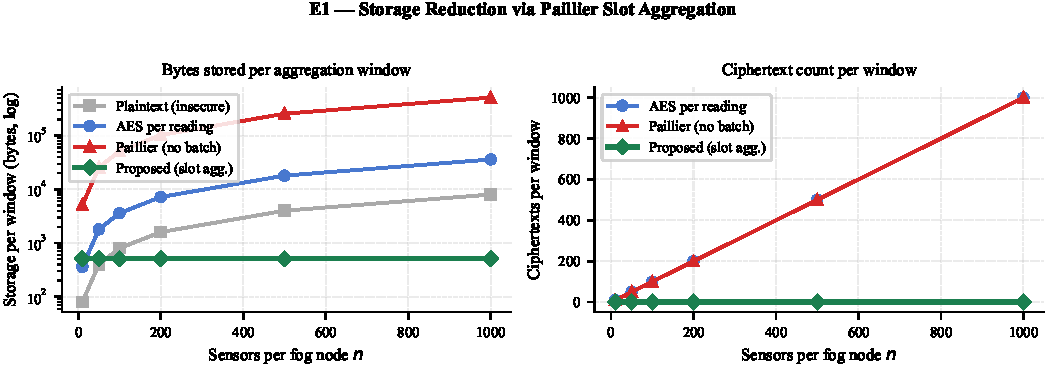
\includegraphics[width=1.0\linewidth]{figures/exp1_storage.pdf}
    \caption{E1: Storage comparison across schemes as a function of sensor count $n$. The upper panel shows total bytes; the lower panel shows ciphertext count. The proposed method stores one ciphertext per window for all $n$.}
    \label{fig:e1-storage}
    \end{figure}

    \subsection{E2: Aggregation Latency with 2048-bit Calibration}
    \label{sec:eval-e2}

    \textbf{Objective.} Characterize the proposed aggregation pipeline using the calibrated 2048-bit cryptographic benchmark and report the component-level contribution of fog conversion, host aggregation, and storage preparation.

    \textbf{Setup and baselines.} For $n\in\{10,50,100,200,500\}$ sensors per window, plaintext summation and AES-GCM encrypt-then-decrypt are measured directly in Python. The Paillier stages of the proposed path use the calibrated \texttt{secure\_iiot\_full\_crypto\_bench 100 2048} mean timings: fog TA conversion $227.537$~ms, host aggregate/KMM combine $1.474$~ms, and storage TA preparation $215.117$~ms. The benchmark uses 2048-bit Paillier ciphertexts of 512~bytes in \texttt{host\_reference\_2048\_no\_ta} mode.

    \textbf{Results.} Fig.~\ref{fig:e2-latency} shows the latency results. Plaintext summation and AES-GCM encryption remain negligible relative to the cryptographic stages. The calibrated proposed path requires $444.128$~ms in total, composed of $227.537$~ms for fog TA conversion, $1.474$~ms for host aggregation/KMM combine, and $215.117$~ms for storage TA preparation. This is within the 500~ms aggregation window. These values are host-reference OP-TEE QEMU benchmark values; they must not be interpreted as physical hardware timings or as TA-side 2048-bit Paillier execution.

    \textbf{Key takeaway.} The calibrated 2048-bit reference places the proposed path within the 500~ms window, while showing that fog conversion and storage preparation dominate the latency budget.

    \begin{figure}[htbp]
    \centering
    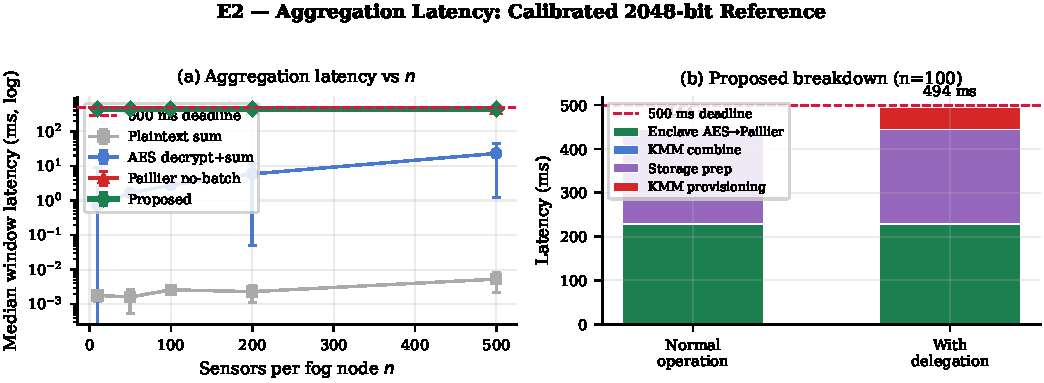
\includegraphics[width=1.0\linewidth]{figures/exp2_latency.pdf}
    \caption{E2: Aggregation latency vs sensor count $n$ with calibrated 2048-bit host-reference Paillier timings. The dashed line marks the 500~ms window. The right panel shows the calibrated component breakdown of the proposed method.}
    \label{fig:e2-latency}
    \end{figure}

    \subsection{E3: Slot Protocol Arithmetic Correctness Under Delegation}
    \label{sec:eval-e3}

    \textbf{Objective.} Verify that the Paillier slot protocol produces numerically correct aggregates when delegation occurs mid-window, for both single-source and multi-source delegation configurations.

    \subsubsection{E3a: Single-Source Delegation}
    \textbf{Setup.} A window of $n=100$ sensors is simulated with $k\in\{1,5,10,20,50\}$ sensors randomly delegated mid-window from primary node $F_1$ to backup node $F_4$. For each of 100 independent trials, the true scaled integer aggregate is computed directly from plaintext readings, and the output of the full slot protocol---AES-to-Paillier enclave conversion, Paillier accumulation with zero-fill for vacated slots, KMM combine, and decryption---is compared against it.

    \textbf{Results.} Across all values of $k$ and all 100 trials, the slot protocol produces zero scaled-integer error. A residual quantization error of approximately 0.045 (median absolute deviation from the true floating-point sum) is observed due to fixed-point integer encoding with $scale=1000$ and is consistent across all delegation counts. This is an inherent property of integer Paillier encoding rather than a protocol defect, and its magnitude is inversely proportional to the scaling factor.

    \subsubsection{E3b: Multi-Source Delegation}
    The protocol is further evaluated under simultaneous delegation from two sources ($F_1$ and $F_2$, each with 30 sensors) to a single backup node ($F_4$ with 30 own sensors), with 5 sensors per source delegated to $F_4$, for 100 independent trials. All 100 trials produce the correct scaled aggregate. The median quantization error is 0.041, consistent with the single-source case.

    \textbf{Key takeaway.} The Paillier slot protocol maintains aggregate correctness under mid-window delegation for both single and multi-source configurations across all 100 trials at every delegation count tested. These results constitute an arithmetic sanity check of the protocol implementation; they do not constitute a cryptographic proof of zero-fill ciphertext indistinguishability, which is argued analytically.

    \begin{figure}[htbp]
    \centering
    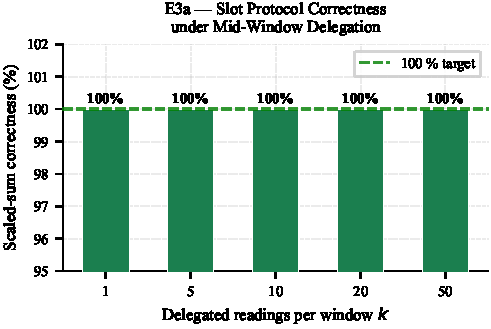
\includegraphics[width=1.0\linewidth]{figures/exp3a_correctness.pdf}
    \caption{E3a: Slot protocol correctness vs delegation count $k$ (100 trials, $n=100$ sensors). The upper panel shows 100\% accuracy at all $k$; the lower panel shows the quantization error due to fixed-point encoding with $scale=1000$.}
    \label{fig:e3a-correctness}
    \end{figure}

    \subsection{E4: KMM Window-Combine Overhead}
    \label{sec:eval-e4}

    \textbf{Objective.} Characterize the latency of the KMM homomorphic window-combine operation as the number of participating fog nodes $k$ increases from 1 to 100.

    \textbf{Setup.} For $k\in\{1,2,5,10,20,50,100\}$ fog aggregates, the KMM combine stage uses the calibrated host aggregate timing from \texttt{secure\_iiot\_full\_crypto\_bench 100 2048}. The measurement is reported as a 2048-bit host-reference benchmark in \texttt{host\_reference\_2048\_no\_ta} mode. Each aggregate ciphertext is 512~bytes at the 2048-bit key size.

    \textbf{Results.} Fig.~\ref{fig:e4-kmm} shows the calibrated host aggregate/KMM combine reference. The combine stage requires $1.474$~ms and remains well within the 500~ms window budget across the tested fog-aggregate counts. The KMM input size still scales linearly with $k$, from 512~bytes at $k=1$ to 51.2~KB at $k=100$.

    \textbf{Key takeaway.} The calibrated KMM combine step contributes only $1.474$~ms, so it is not the limiting factor in the 500~ms aggregation window.

    \begin{figure}[htbp]
    \centering
    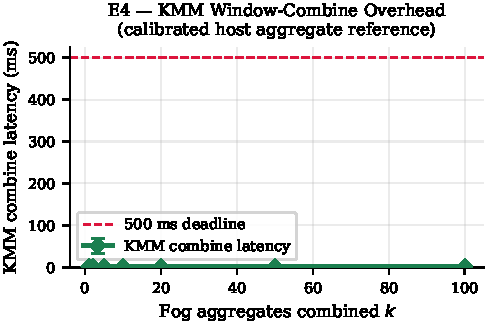
\includegraphics[width=1.0\linewidth]{figures/exp4_kmm_combine.pdf}
    \caption{E4: KMM window-combine latency vs number of fog aggregates $k$ using the calibrated 2048-bit host aggregate reference. The dashed line marks 500~ms. The right panel shows total bytes received by the KMM at each $k$.}
    \label{fig:e4-kmm}
    \end{figure}

    \subsection{E5: Load Balancing Strategy Comparison}
    \label{sec:eval-e5}

    \textbf{Objective.} Compare the proposed CapacityScore strategy against five delegation baselines under heterogeneous fog capacity, bursty task arrivals, and a temporary fog-node failure.

    \textbf{Setup and baselines.} The E5 simulator uses five fog nodes with heterogeneous CPU, RAM, bandwidth, latency, and processing-rate factor $\phi$: $F_1$ and $F_5$ are high-capacity low-latency nodes, $F_2$ and $F_4$ are medium-capacity nodes, and $F_3$ is the slowest node. Each run spans 20 aggregation windows of 500~ms. The workload phases are normal operation (W1--5), an $F_1$ burst (W6--10), $F_5$ failure (W11--13), recovery (W14--17), and an $F_4$ burst (W18--20). Tasks are generated from two classes: latency-sensitive (LS) tasks with 100~ms deadlines and heavy-processing (HP) tasks with 500~ms deadlines. Each fog group has a fixed HP/LS mix, creating CPU-heavy, bandwidth-heavy, and LS-only primary identities.

    For the CapacityScore normalization (Eq.~\eqref{eq:e5-normalized-latency-queue}), the latency ceiling is set to $lat_j^{cap} = 40\,\text{ms}$, matching the configured latency of $F_3$, the slowest node in this experiment. Queue occupancy is tracked by the gossip protocol as a pre-normalized fraction in $[0,1]$.

    Six strategies are compared. S1 chooses uniformly at random from candidates; S2 uses a persistent round-robin index; S3 selects the candidate with minimum $Workload(F_j)$; S4 uses fixed CapScore weights; S5 uses task-adaptive weights without a compatibility term; and S6 is the proposed CapacityScore with the compatibility term. Their scoring functions are:

    \begin{equation}
    \begin{aligned}
    score_{S4}(F_j) ={}& 0.50(1-Workload(F_j)) \\
    &+ 0.15(1-\ell_j) \\
    &+ 0.35(1-q_j)
    \end{aligned}
    \label{eq:s4-score}
    \end{equation}

    \begin{equation}
    \begin{aligned}
    score_{S5}(F_j,t_{type}) ={}& w_1(1-Workload(F_j)) \\
    &+ w_2(1-\ell_j) \\
    &+ w_3(1-q_j)
    \end{aligned}
    \label{eq:s5-score}
    \end{equation}

    \begin{equation}
    score_{S6}(F_j,t_{type}) = CapacityScore(F_j,t_{type})
    \label{eq:s6-score}
    \end{equation}

    S4 applies fixed weights $(w_1,w_2,w_3)=(0.50,0.15,0.35)$ with no compatibility term. S5 adapts the weights by task type but also omits the compatibility term. S6 adds the task-type compatibility term: LS routing prioritizes bandwidth availability, while HP routing applies a $\phi^2$ penalty to structurally disfavor slow nodes for compute-heavy tasks. Results are averaged over 20 seeds $\{42,\ldots,61\}$ with 95\% confidence intervals.

    \textbf{Metrics.} The reported metrics are completion rate, deadline satisfaction rate, delegation rate, re-delegation rate, mean waiting time, workload standard deviation, resource-utilization standard deviations, per-task-type deadline miss rates, and phase-level deadline satisfaction.

    \textbf{Results.} Aggregate results are shown in Fig.~\ref{fig:e5-delegation-quality} and Fig.~\ref{fig:e5-resource-std}. All six strategies complete 100\% of tasks, so the discriminating metrics are deadline satisfaction and routing quality. S6 achieves the highest overall deadline satisfaction, 78.77\% ($\pm$0.88\%), followed by S5 at 78.35\% ($\pm$0.88\%), S3 at 77.28\% ($\pm$0.79\%), S4 at 77.01\% ($\pm$0.70\%), S2 at 63.34\% ($\pm$0.52\%), and S1 at 63.10\% ($\pm$0.61\%). The 0.42 percentage-point margin between S6 and S5 lies within the reported confidence intervals; the advantage of the compatibility term is more conclusively demonstrated by the per-task-type and bandwidth-balance metrics reported below. S6 also has the lowest mean waiting time, 101.11~ms ($\pm$3.94~ms), compared with 103--104~ms for S3--S5 and approximately 790--854~ms for S1--S2. The proposed S6 strategy delegates fewer tasks than the other informed strategies, 43.87\% ($\pm$1.21\%) versus 47.99--49.19\% for S3--S5, and no strategy produces re-delegation in this simulator configuration.

    Resource-balance results show the effect of the compatibility term. S6 has the lowest bandwidth-utilization standard deviation, $\sigma_{BW}=0.225$ ($\pm$0.005), compared with 0.239 for S5, 0.250 for S3, 0.251 for S4, and 0.363 for S1--S2. The time-series view in Fig.~\ref{fig:e5-sigma-bw-ts} shows the same behavior across the burst, failure, and recovery phases. S6 does not minimize the scalar workload standard deviation because it intentionally avoids using structurally incompatible capacity; its mean workload standard deviation is 0.167, while S3--S5 are approximately 0.155--0.156. This is an expected tradeoff: S6 accepts slightly less even scalar workload distribution to reduce deadline misses and bandwidth imbalance.

    The task-type breakdown in Fig.~\ref{fig:e5-task-type} and Fig.~\ref{fig:e5-hp-f3} explains the deadline improvement. HP tasks miss deadlines at 15.18\% under S6, compared with 17.70\% for S4, 18.59\% for S3, 18.67\% for S5, and about 34--35\% for S1--S2. S6 assigns only 1.97\% of HP tasks to $F_3$, while S3--S5 assign 3.32--3.77\% and S1--S2 assign approximately 13.8--14.0\%. Because $F_3$ executes HP tasks in 600~ms, exceeding the HP deadline, reducing HP placement on $F_3$ directly reduces deadline failures. Phase-level results in Fig.~\ref{fig:e5-phase-deadline} show that S6 is strongest during normal operation (92.67\%), recovery (93.83\%), and the $F_4$ burst phase (84.51\%). During $F_5$ failure, S5 performs best (48.22\%) while S6 drops to 37.93\%. This is an expected consequence of the compatibility-heavy weighting ($w_4=0.45$): when node failure reduces the candidate pool, S6's structural selectivity narrows choices further than S5's load-only ranking. Deployments anticipating simultaneous node failure and high task arrival rates may consider reducing $w_4$ during degraded-mode operation to recover broader candidate coverage.

    \textbf{Key takeaway.} E5 shows that CapacityScore improves deadline satisfaction primarily by routing HP tasks away from structurally incompatible nodes and by reducing bandwidth-utilization variance. The result is not a completion-rate improvement, since every strategy completes all tasks in this configuration; it is a deadline and routing-quality improvement under heterogeneous fog capacity and phased stress.

    \begin{figure}[htbp]
    \centering
    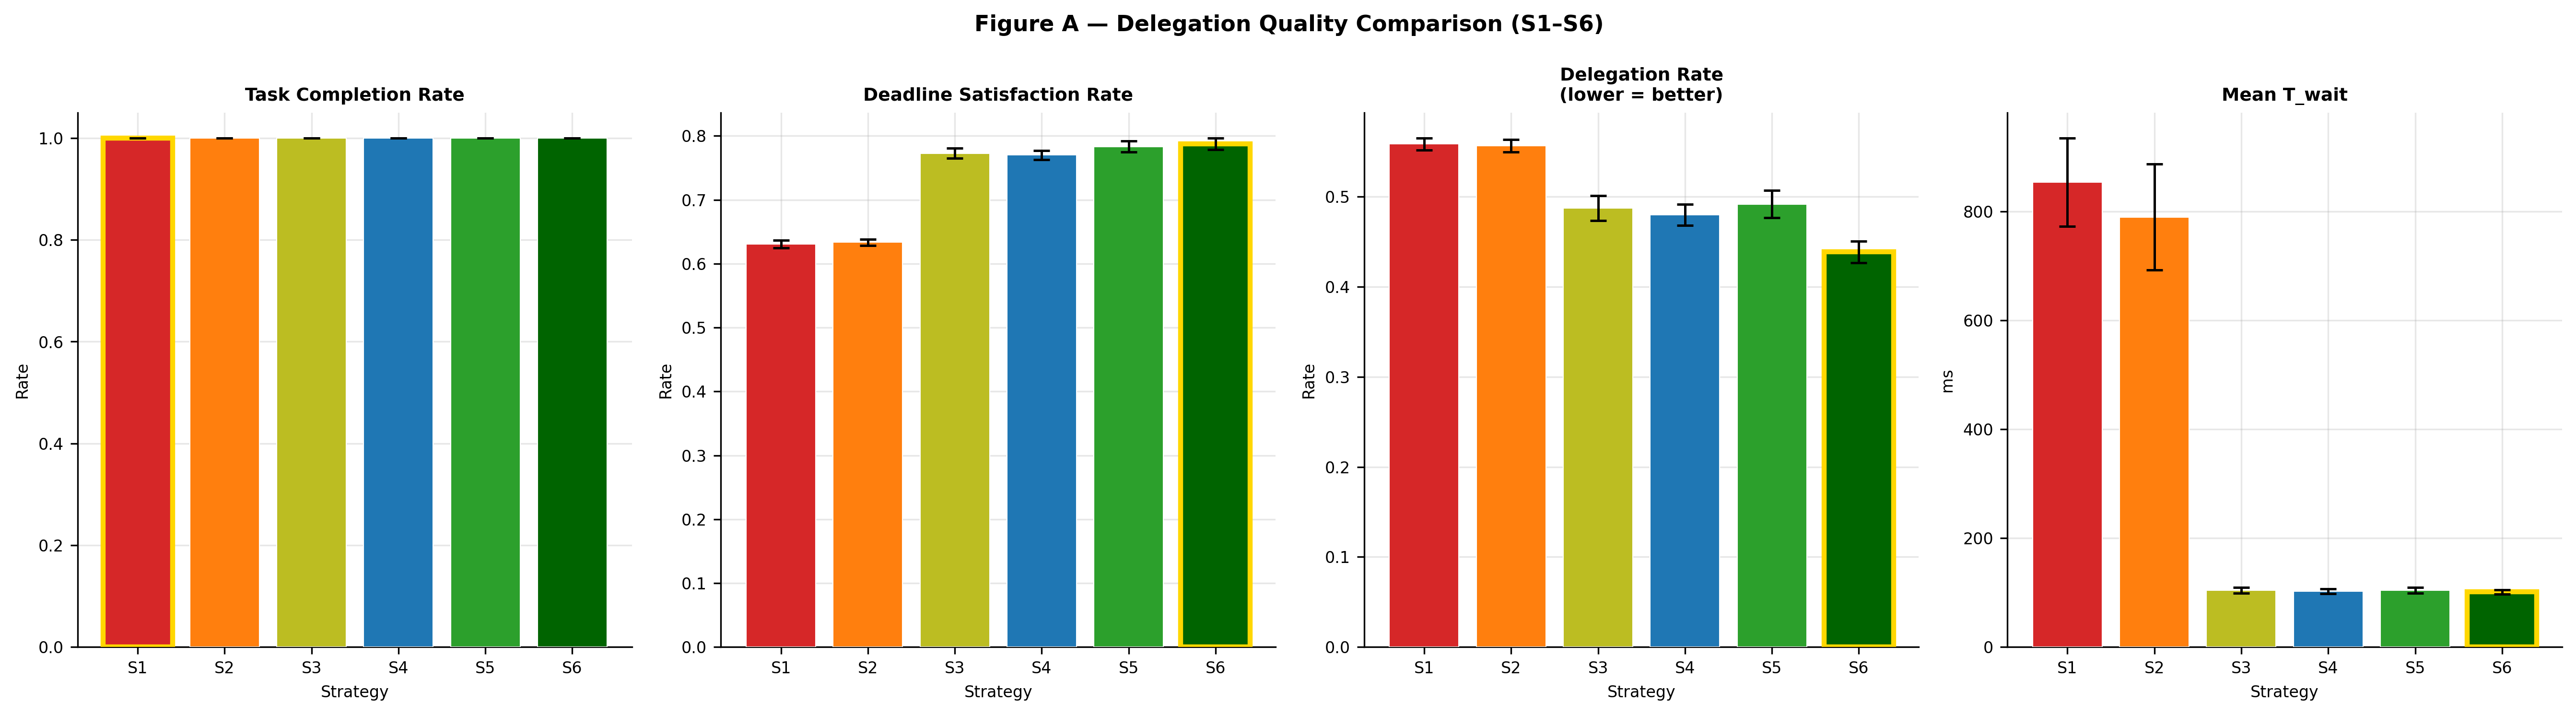
\includegraphics[width=1.0\linewidth]{figures/e5_figA_delegation_quality.png}
    \caption{E5 Figure A: delegation quality across S1--S6. Panels report completion rate, deadline satisfaction rate, delegation rate, and mean waiting time over 20 seeds with 95\% CI.}
    \label{fig:e5-delegation-quality}
    \end{figure}

    \begin{figure}[htbp]
    \centering
    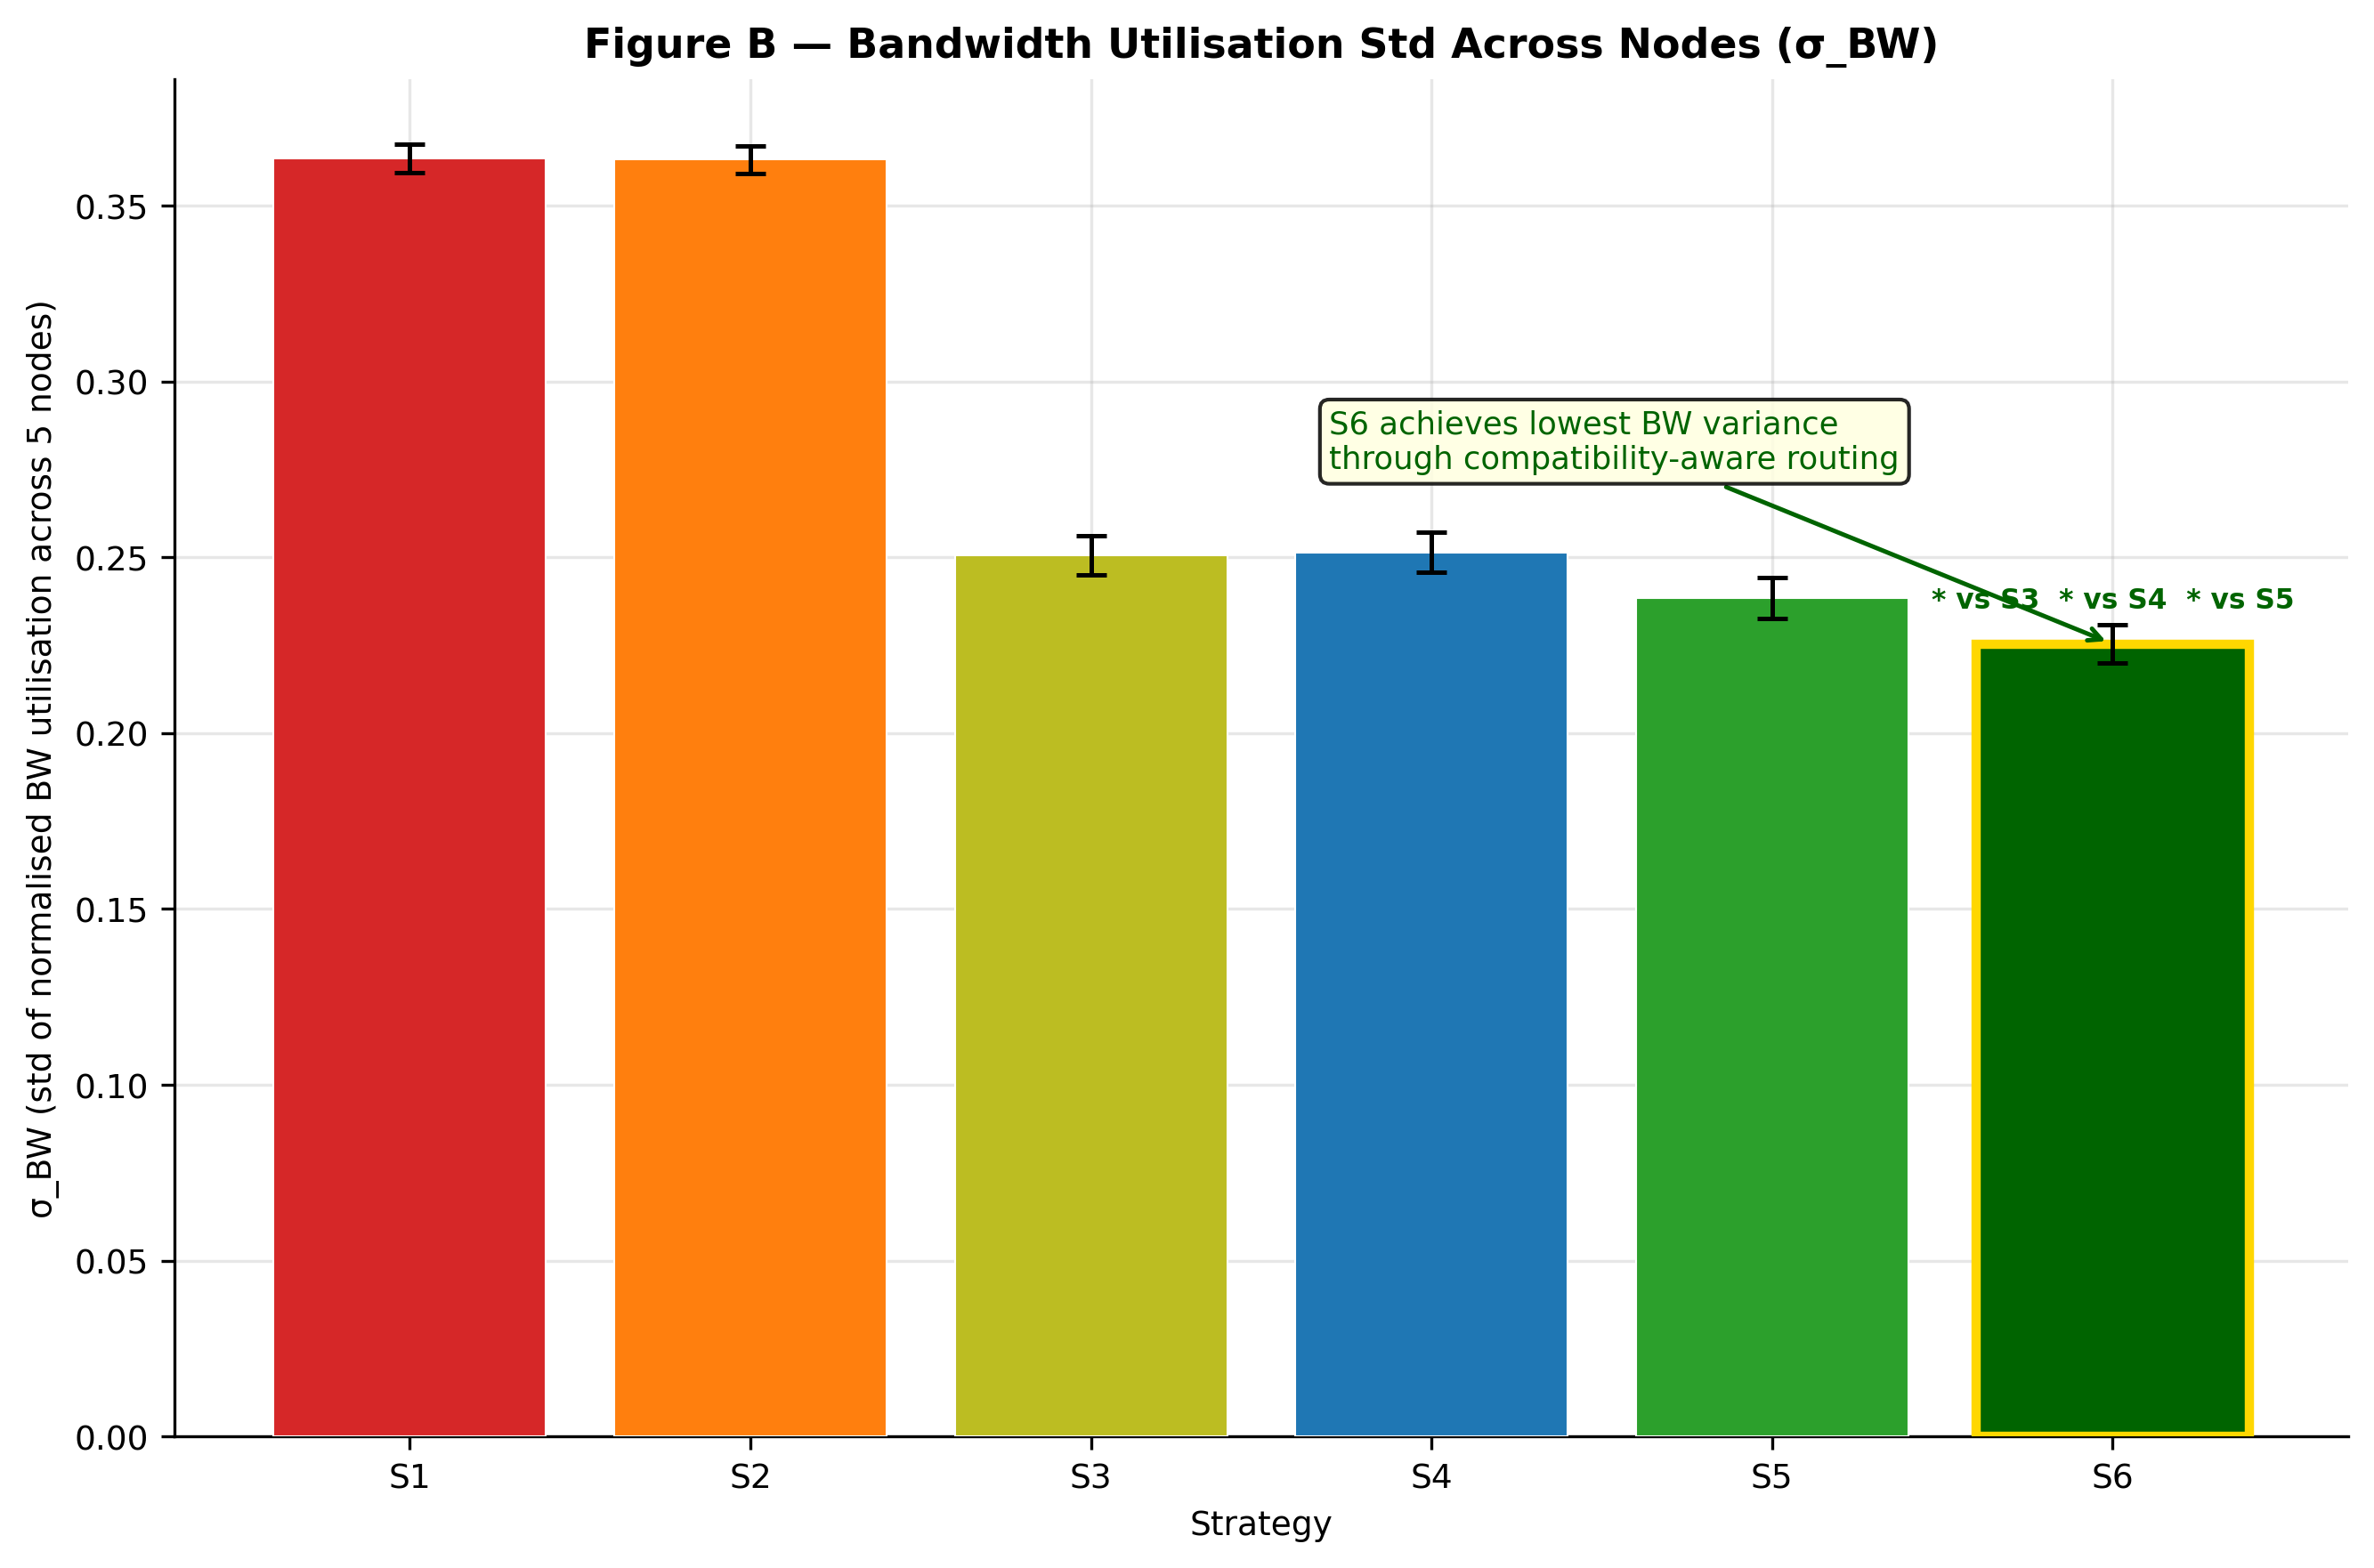
\includegraphics[width=0.9\linewidth]{figures/e5_figB_resource_util_std.png}
    \caption{E5 Figure B: bandwidth-utilization standard deviation across fog nodes. Lower $\sigma_{BW}$ indicates more stable bandwidth distribution.}
    \label{fig:e5-resource-std}
    \end{figure}

    \begin{figure}[htbp]
    \centering
    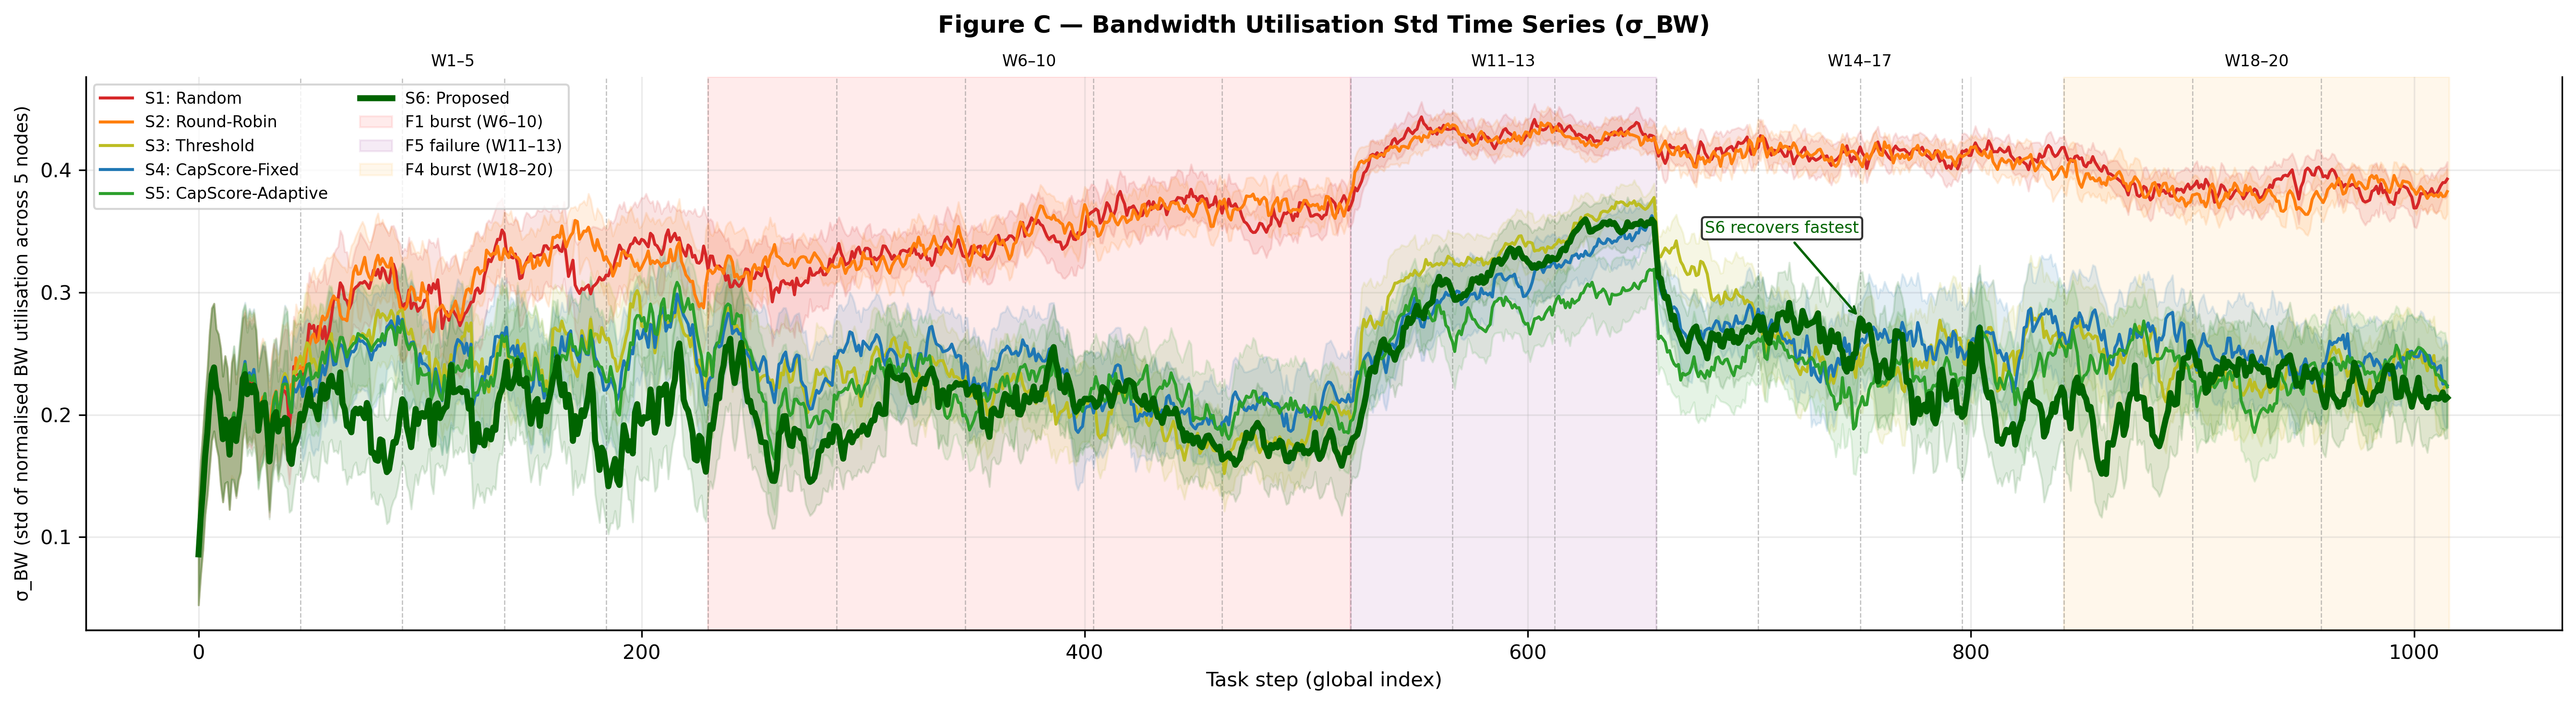
\includegraphics[width=1.0\linewidth]{figures/e5_figC_sigma_bw_timeseries.png}
    \caption{E5 Figure C: $\sigma_{BW}$ time series across normal, burst, failure, recovery, and second-burst phases. Shaded bands mark stress and failure intervals.}
    \label{fig:e5-sigma-bw-ts}
    \end{figure}

    \begin{figure}[htbp]
    \centering
    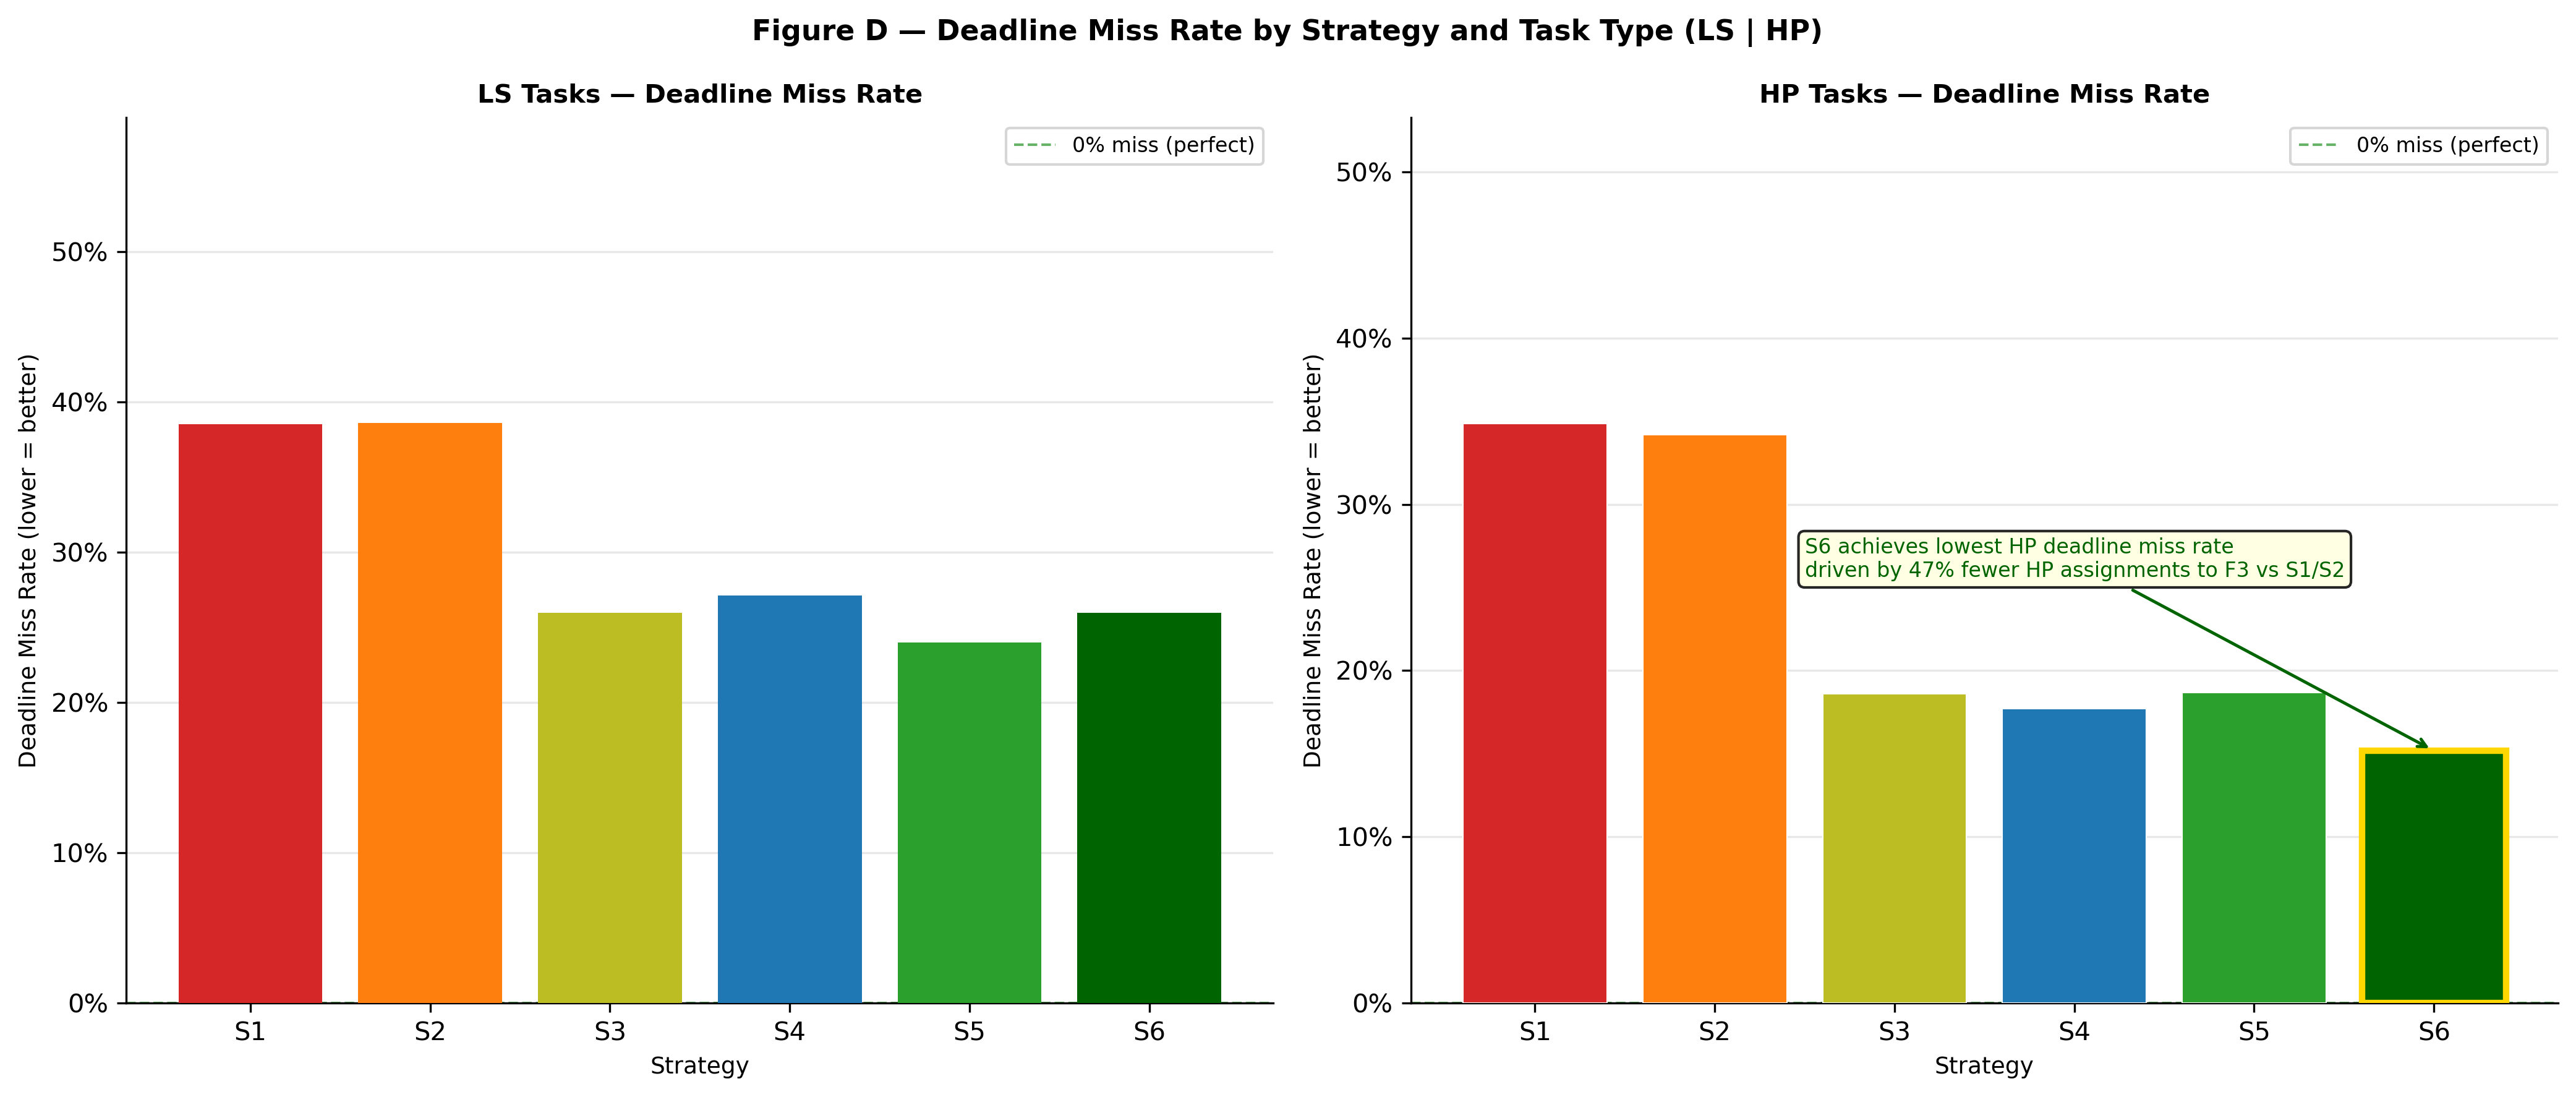
\includegraphics[width=1.0\linewidth]{figures/e5_figD_ttotal_boxplots.png}
    \caption{E5 Figure D: deadline miss rate by task type. S6 reduces HP misses by avoiding structurally slow HP placements.}
    \label{fig:e5-task-type}
    \end{figure}

    \begin{figure}[htbp]
    \centering
    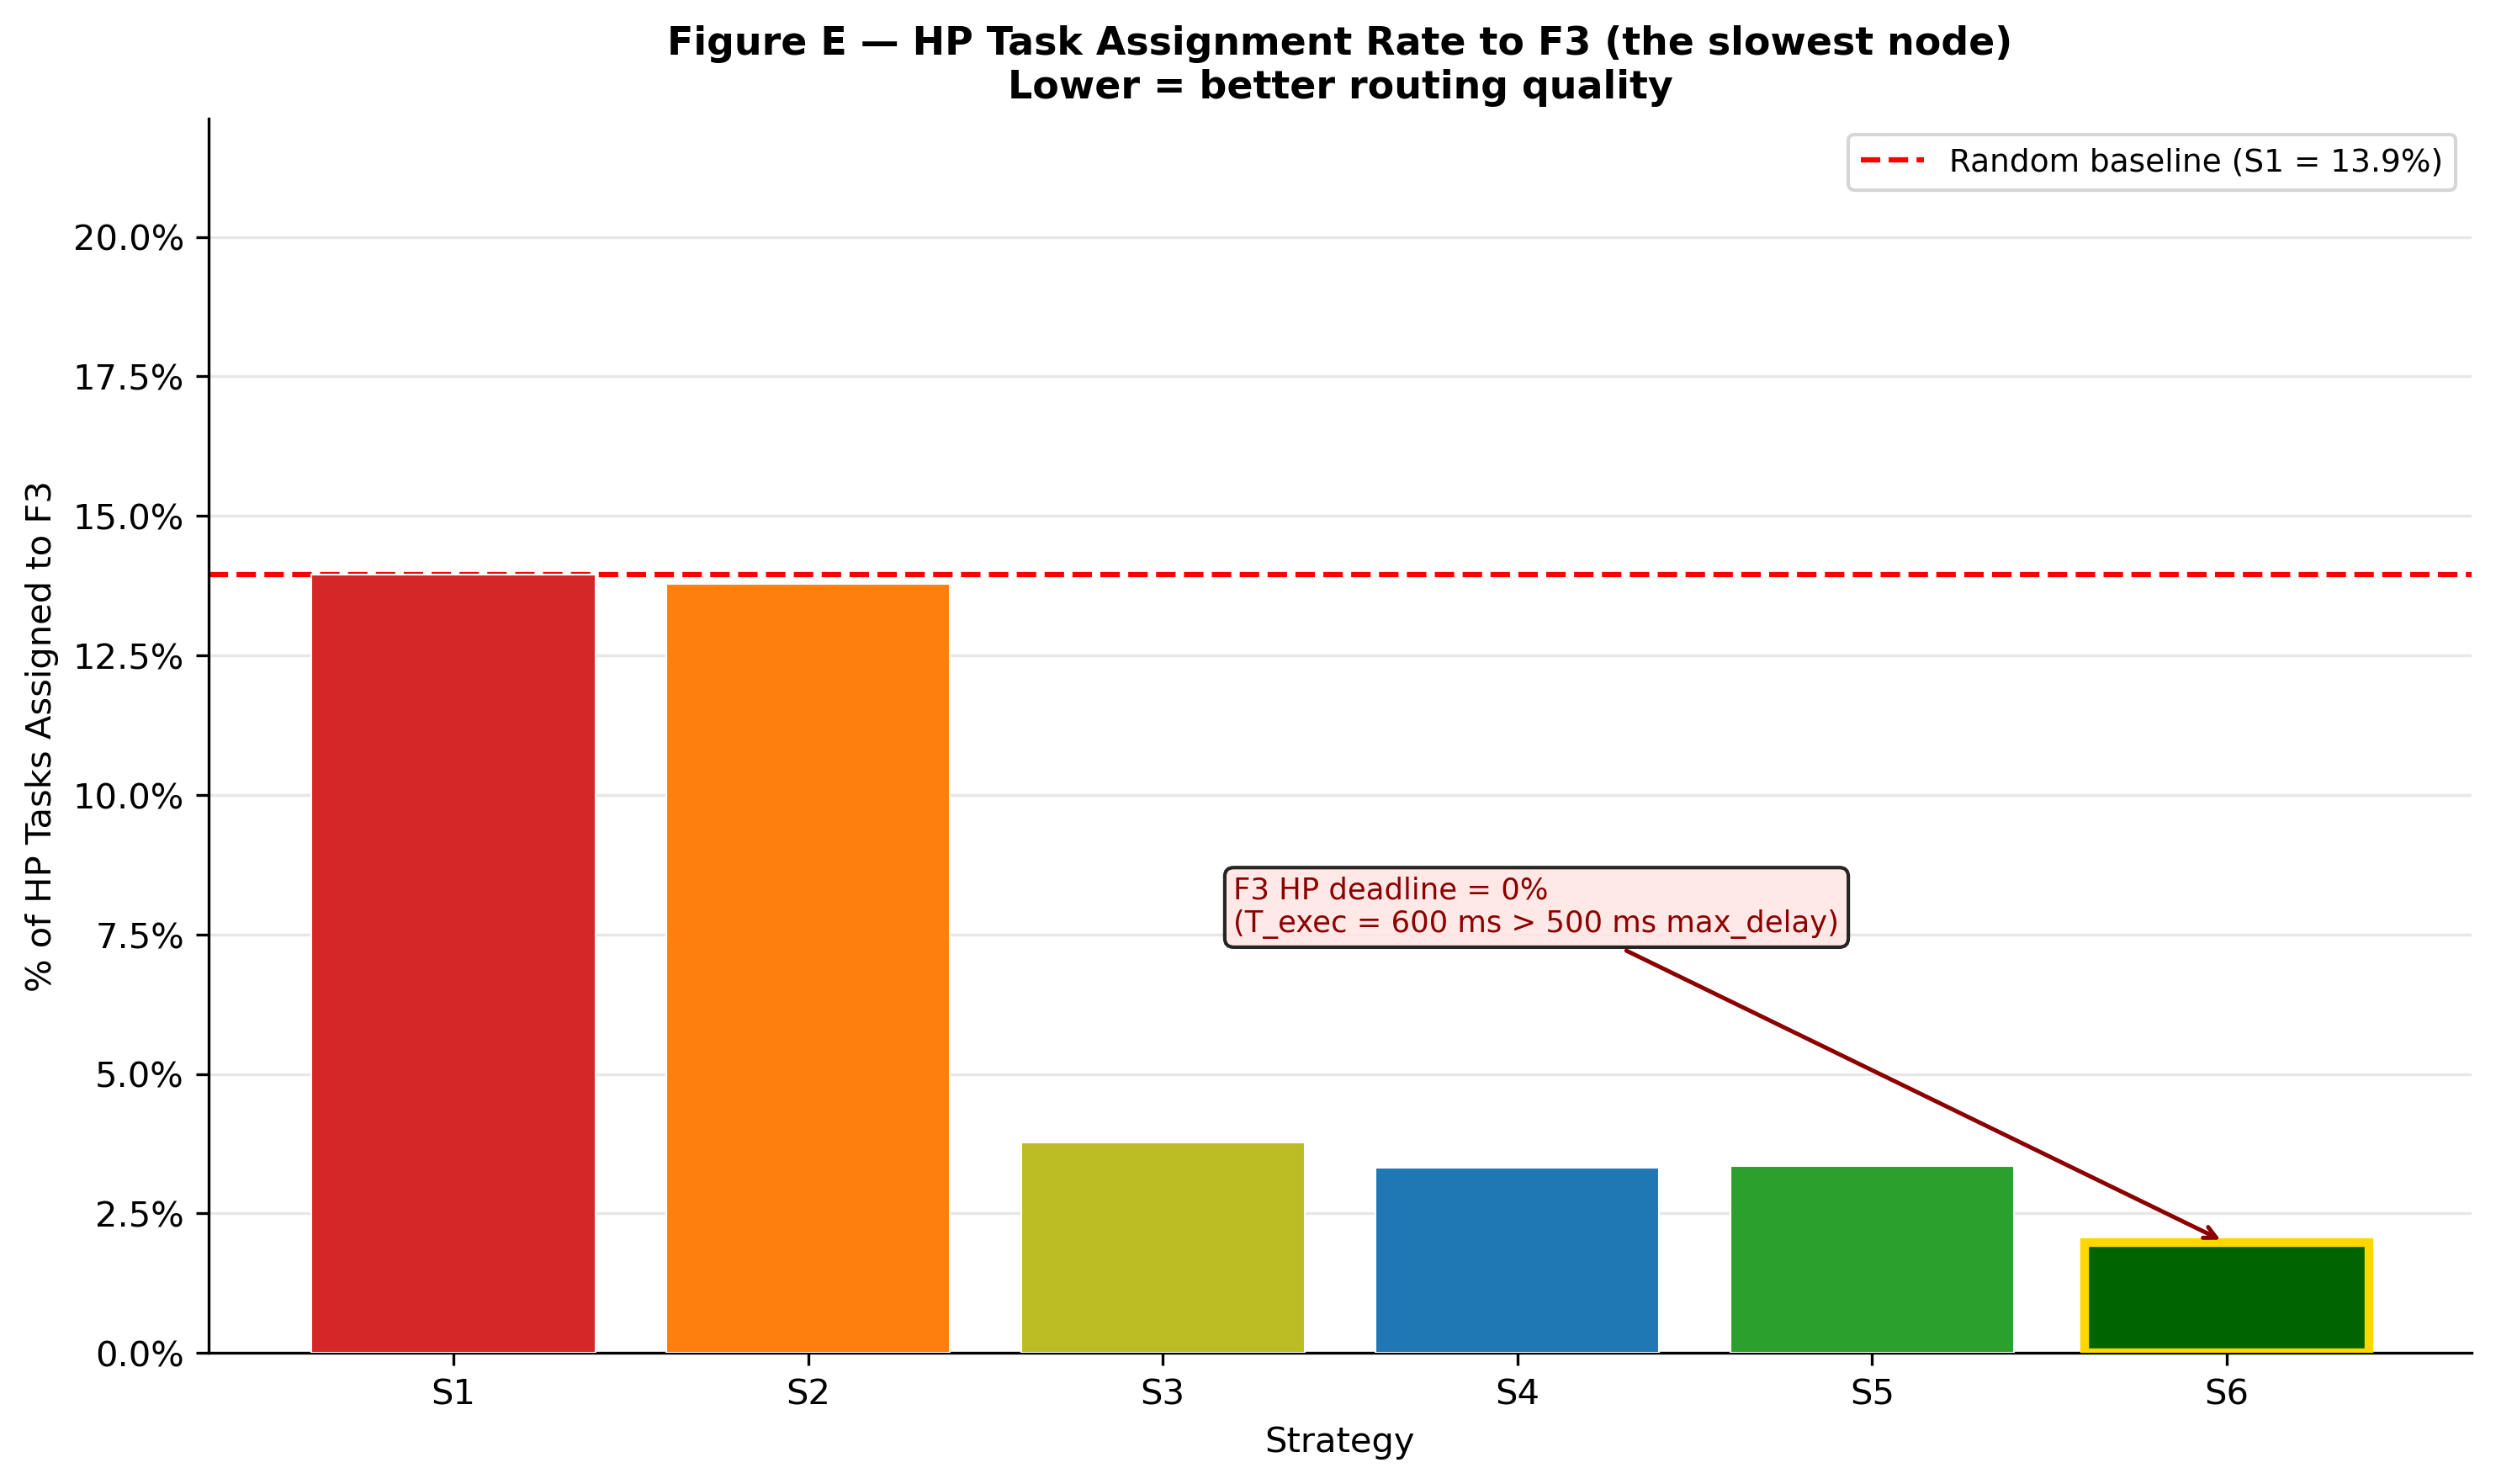
\includegraphics[width=0.9\linewidth]{figures/e5_figE_node_scatter_w8.png}
    \caption{E5 Figure E: HP assignment rate to $F_3$, the slowest and HP-incompatible node. Lower values indicate better task-aware routing.}
    \label{fig:e5-hp-f3}
    \end{figure}

    \begin{figure}[htbp]
    \centering
    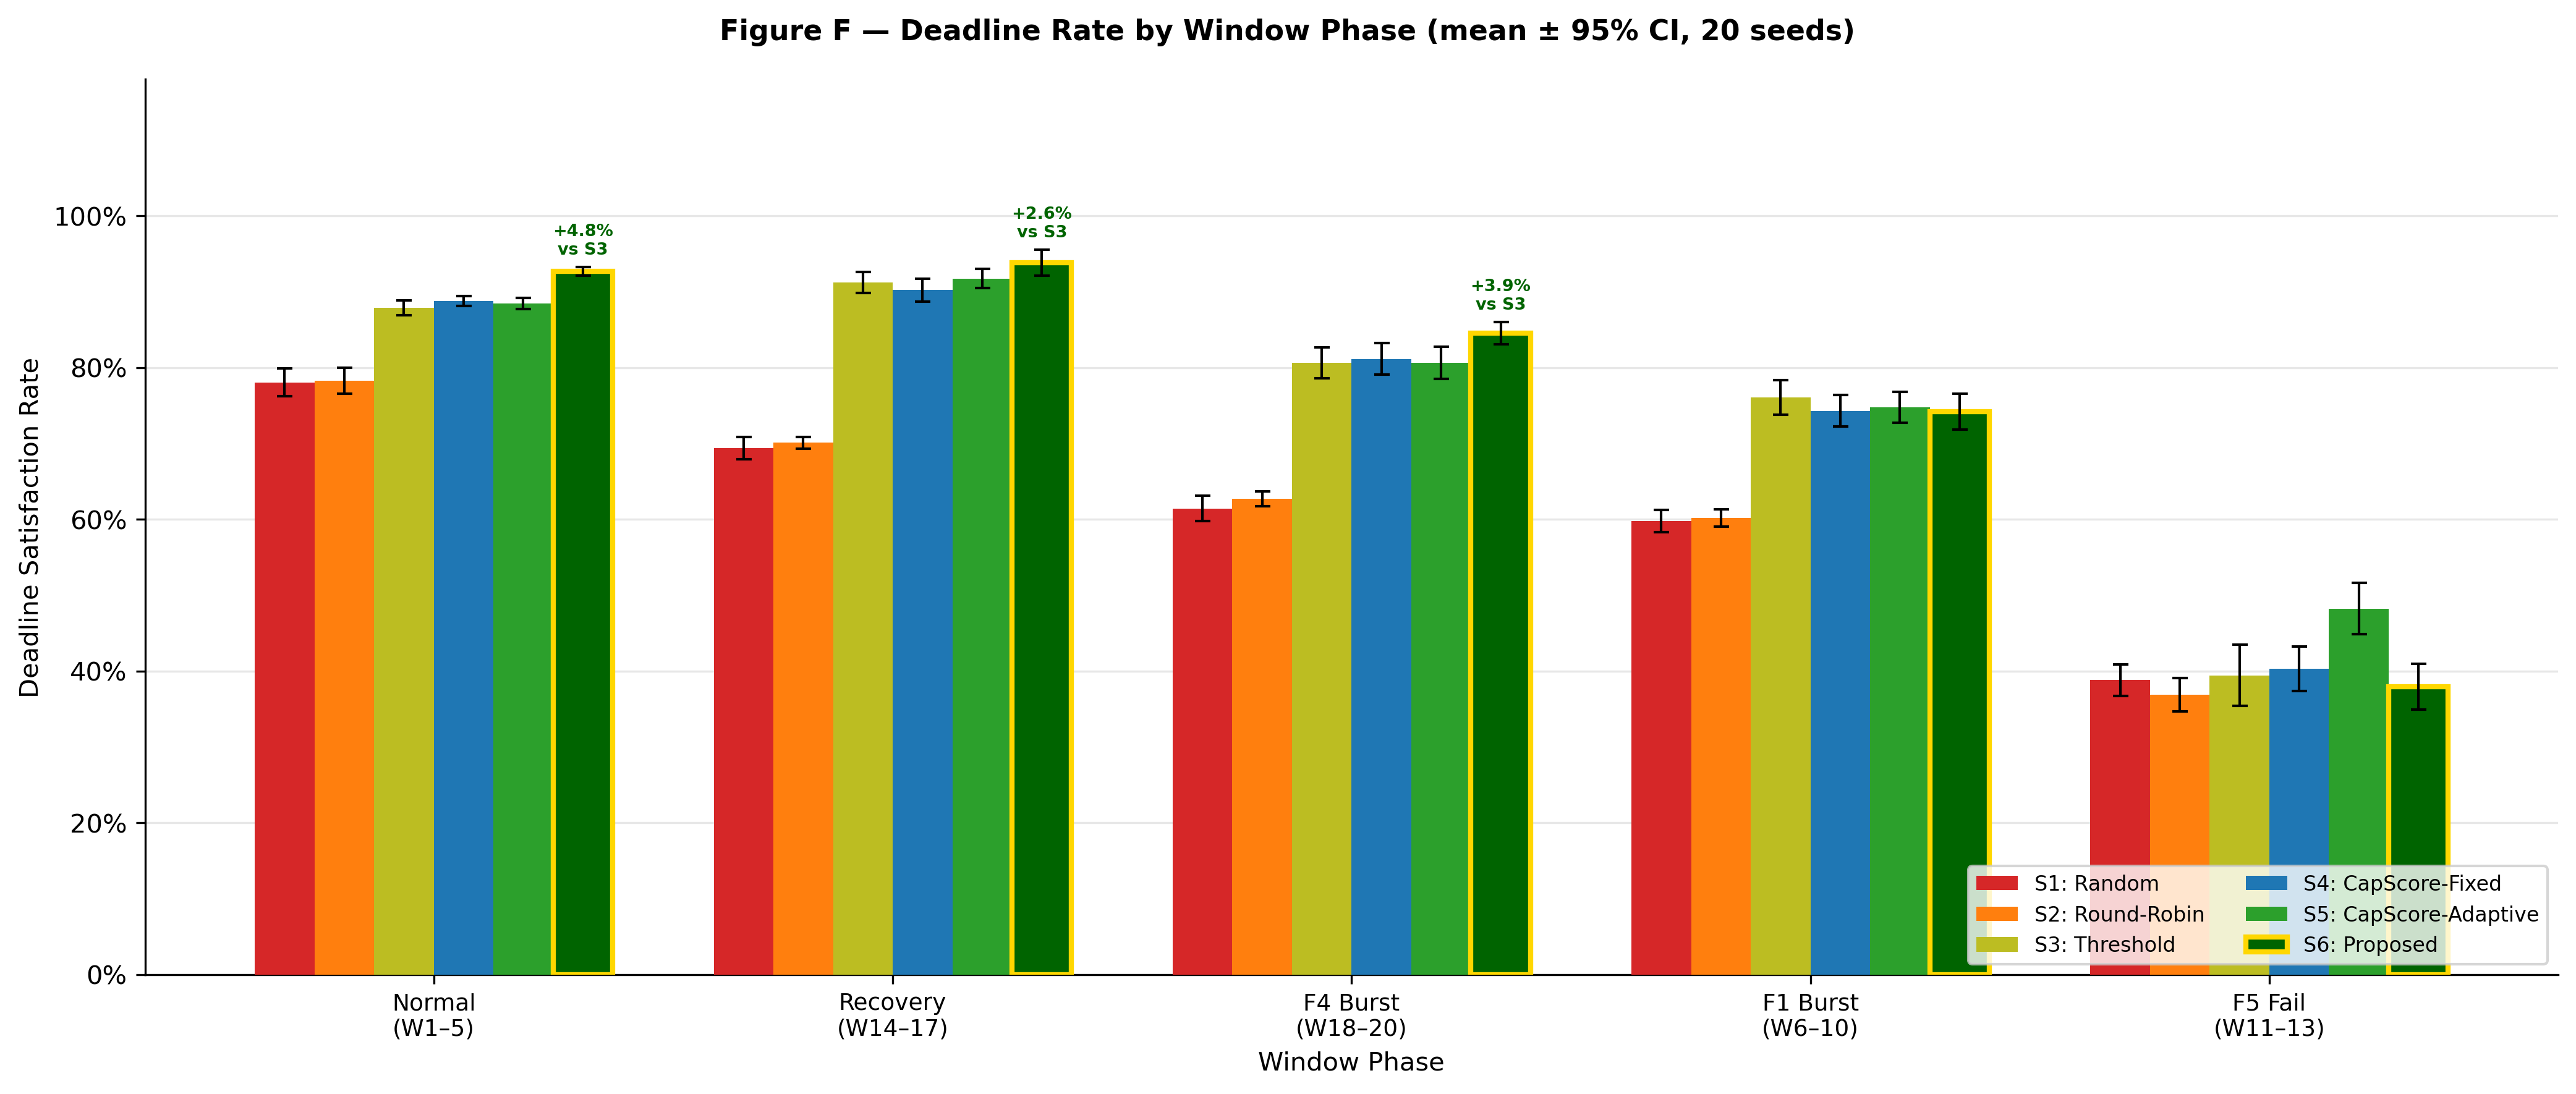
\includegraphics[width=1.0\linewidth]{figures/e5_figF_phase_deadline.png}
    \caption{E5 Figure F: phase-level deadline satisfaction over 20 seeds with 95\% CI.}
    \label{fig:e5-phase-deadline}
    \end{figure}

    \subsection{E6: Fault Detection and Recovery Analysis}
    \label{sec:eval-e6}

    \textbf{Objective.} Evaluate data loss rate and recovery latency of the proposed ACK+KMM fault recovery mechanism against five representative baselines across three failure timing scenarios.

    \textbf{Setup and baselines.} An analytical reading-loss model is evaluated over 30 simulation seeds and three failure scenarios: failure at the start of the observation window (\textit{fail\_0ms}), failure at 250~ms (\textit{mid\_window}), and failure at 450~ms (\textit{late\_window}). The observation period spans 2000~ms (four 500~ms windows), during which 400 readings are generated in total (100 per 500~ms window, one per sensor). The compared baselines are derived from representative fault-tolerance mechanisms reported in the literature, but they are implemented as simulator-level abstractions rather than complete reproductions of the cited systems. This distinction is important because the original studies differ in architecture, workload, and optimization objective.

    Table~\ref{tab:e6-baselines} summarizes the five baselines used in E6. B1 is the direct gossip-only baseline used by the proposed architecture, where a fog failure is detected only after $r{=}3$ missed gossip rounds, giving $rT_g=3\times500\,\text{ms}=1500\,\text{ms}$. During this interval, readings addressed to the failed fog node are counted as lost. B2 abstracts replica-based fog fault tolerance, following the principle that task reliability can be improved by executing replicas on alternative fog resources~\cite{liu2024replica}; in the simulator, each sensor reading is sent simultaneously to a primary and backup fog node, so data loss is zero under a single primary failure but message and compute units are doubled. B3 abstracts checkpoint/recovery mechanisms used in resilient cloud and service-function-chain management~\cite{shahab2025sfc}; the simulator models periodic checkpoints at 500~ms intervals and a 500~ms restore interval, so readings after the latest checkpoint and before recovery completion may be unavailable. B4 is based on multilayer liveness detection, where multiple detector layers are combined to reduce fault detection time compared with a single heartbeat detector~\cite{lee2022multilayer}; the simulator represents this idea using independent sensor, fog, and KMM-layer checks and uses the earliest active detection result. B5 is based on fog/SIoT clustering fault tolerance, where clusters and standby resources support fault detection and recovery~\cite{mohammadi2023fsiot}; the simulator models a cluster coordinator that detects the failed fog node, selects a replacement, and reroutes subsequent readings.

    \begin{table}[htbp]
    \centering
    \caption{E6 Literature-Derived Fault-Tolerance Baselines}
    \label{tab:e6-baselines}
    \begin{tabular}{p{0.12\linewidth}p{0.28\linewidth}p{0.47\linewidth}}
    \toprule
    Baseline & Reference role & Simulator abstraction \\
    \midrule
    B1 & Direct gossip-only baseline & Failure detected after $rT_g=1500\,\text{ms}$; readings sent to the failed fog before detection are lost. \\
    B2 & Replica-based fog fault tolerance~\cite{liu2024replica} & Each reading is sent to both primary and backup fog nodes; backup output is used after primary failure. \\
    B3 & Checkpoint/recovery baseline~\cite{shahab2025sfc} & A checkpoint is written periodically; recovery resumes from the latest checkpoint after a restore delay. \\
    B4 & Multilayer liveness detection~\cite{lee2022multilayer} & Sensor, fog, and KMM-layer detectors operate independently; detection uses the earliest active layer result. \\
    B5 & Fog-clustering fault tolerance~\cite{mohammadi2023fsiot} & A cluster coordinator detects the failed fog, selects a replacement, and reroutes later readings. \\
    \bottomrule
    \end{tabular}
    \end{table}

    The proposed method uses sensor ACK timeout $T_{ack}{=}100\,\text{ms}$ followed by KMM key provisioning $T_{KMM}{=}50\,\text{ms}$, yielding a modeled recovery latency of 150~ms. The backup fog node is selected using CapacityScore (S6) with the LS weight configuration as the default, since raw sensor ciphertexts carry no task-type metadata (see Section~\ref{sec:lb}). The analytical model treats backup selection as a black box: it assumes the selected node has sufficient residual capacity to accept redirected readings within the $T_{ack}+T_{KMM}$ window; the specific backup node chosen does not affect the reported loss rates or recovery latency. All results are therefore analytical estimates under a common failure-timing model and should not be interpreted as empirical end-to-end measurements of the original baseline systems.

    \textbf{Results.} Fig.~\ref{fig:e6-fault} shows data loss rates and recovery latency across methods. Loss rates are reported as a fraction of the 400-reading observation total; this denominator is held fixed across all methods so that all methods are compared on a common scale. The simulator counts all sensor readings that fall within the failure-to-recovery time window as lost. In the worst-case scenario (failure at $t{=}0$), the proposed method (using CapacityScore S6 with LS-default weight configuration for backup node selection) loses approximately 7.5\% of readings ($\approx$30 of 400 during the 150~ms recovery window), averaged over 30 seeds. Recovery latency is measured from the first missed ACK event, not from the failure instant; worst-case failure-to-detection can be up to one inter-reading interval (125~ms) longer if the node fails immediately after a successful transmission. The proposed method compares with 75\% for B1 gossip (1500~ms outage), 25\% each for B3 checkpoint and B4 multilayer (500~ms detection windows), and approximately 38\% for B5 clustering (750~ms window). B2 replication achieves zero data loss at the cost of doubling message overhead. The proposed method incurs a message overhead of $1.055\times$ the baseline, attributable to per-reading ACK messages and two KMM provisioning messages per recovery event. Fig.~\ref{fig:e6-tradeoff} illustrates the data-loss versus message-overhead tradeoff space; the proposed method is nearest to the origin among single-mechanism approaches.

    \textbf{Key takeaway.} The proposed ACK+KMM mechanism reduces worst-case data loss from 75\% (gossip-only) to approximately 7.5\% while incurring only a 5.5\% increase in message overhead, representing a favorable tradeoff relative to all compared baselines except B2 replication, which achieves zero data loss at $2\times$ message cost.

    \begin{figure}[htbp]
    \centering
    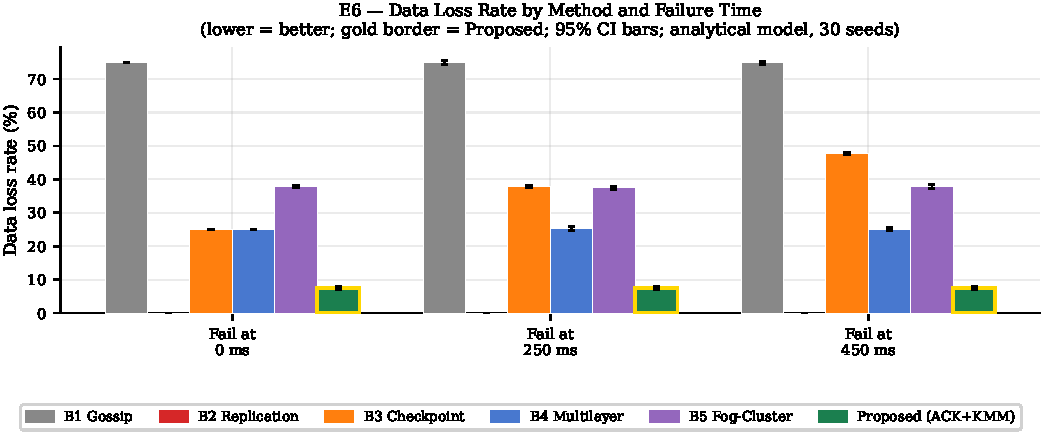
\includegraphics[width=1.0\linewidth]{figures/exp6_data_loss.pdf}
    \caption{E6: Data loss rate (upper) and recovery latency (lower) across six methods and three failure timing scenarios, averaged over 30 seeds with 95\% CI. Results are derived from an analytical reading-loss model.}
    \label{fig:e6-fault}
    \end{figure}

    \begin{figure}[htbp]
    \centering
    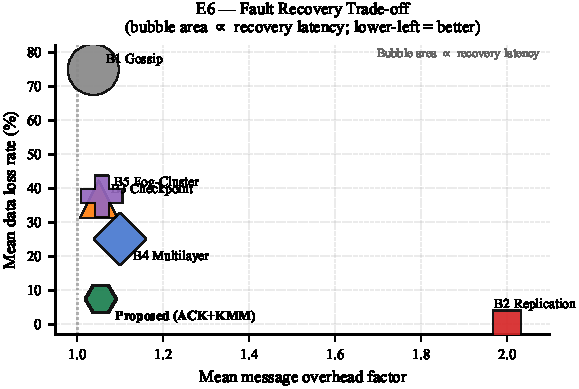
\includegraphics[width=1.0\linewidth]{figures/exp6_tradeoff.pdf}
    \caption{E6: Data loss vs message overhead tradeoff. Each marker represents one method; the proposed ACK+KMM method (green) is closest to the origin in loss--overhead space.}
    \label{fig:e6-tradeoff}
    \end{figure}

    \subsection{E7: End-to-End Pipeline Latency (Analytical Model)}
    \label{sec:eval-e7}

    \textbf{Objective.} Estimate end-to-end latency and per-window storage footprint of the proposed pipeline under hardware-accelerator assumptions and compare against three representative baselines across dynamic window conditions.

    \textbf{Setup and baselines.} The model uses hardware-target latency constants: sensor AES encryption (0.001~ms, hardware AES-NI), Paillier encryption per slot (3.8~ms, hardware-assisted co-processor), Paillier homomorphic addition (0.01~ms), KMM combine inside TEE (1.0~ms), storage preparation (5.0~ms), cloud upload (10.0~ms), and TEE key delegation round-trip (150.0~ms). For $n{=}100$ sensors, four methods are evaluated across the same 20-window schedule as E5: (i)~\emph{cloud-only} (raw sensor values uploaded directly, no fog processing), (ii)~\emph{fog plaintext} (fog accumulates an unencrypted sum; insecure lower bound), (iii)~\emph{Paillier-fog-convert} (per-reading Paillier encryption at the fog, no slot aggregation, one ciphertext per window sent to cloud), and (iv)~\emph{proposed}. These latency constants represent a separate target-deployment analytical model; E2 reports the calibrated 2048-bit host-reference benchmark.

    \textbf{Results.} Fig.~\ref{fig:e7-pipeline} shows pipeline latency and per-window storage. Cloud-only and fog-plaintext complete in 40~ms and 13~ms, respectively; however, cloud-only stores 100 raw values per window (800~bytes) while fog-plaintext provides no data confidentiality. The Paillier-fog-convert baseline requires 393~ms and stores one 512-byte ciphertext per window, satisfying the 500~ms budget across all 20 windows. The proposed method requires 399~ms during non-delegation windows (12 of 20 windows) and 549~ms during delegation windows (8 of 20 windows, corresponding to the F2-overload burst phases W6--10 and W18--20), where the additional 150~ms TEE key delegation step is active. Both the proposed method and the Paillier-fog-convert baseline store one aggregate per window, compared with 100 raw items per window for cloud-only.

    \textbf{Key takeaway.} Under hardware-target assumptions, the proposed method achieves the same aggregate storage efficiency as the Paillier-fog-convert baseline (one ciphertext per window) while additionally supporting delegation and fault recovery. The 500~ms budget is maintained in 12 of 20 windows; delegation windows (W6--10 and W18--20) incur an additional 150~ms, which is the cost of TEE key provisioning. Systems deploying the proposed scheme should account for this delegation overhead in capacity planning, either by provisioning sufficient headroom or by extending the aggregation window during anticipated burst phases. The fog-plaintext baseline serves as a latency lower bound only and does not satisfy the confidentiality requirements of the proposed threat model.

    \begin{figure}[htbp]
    \centering
    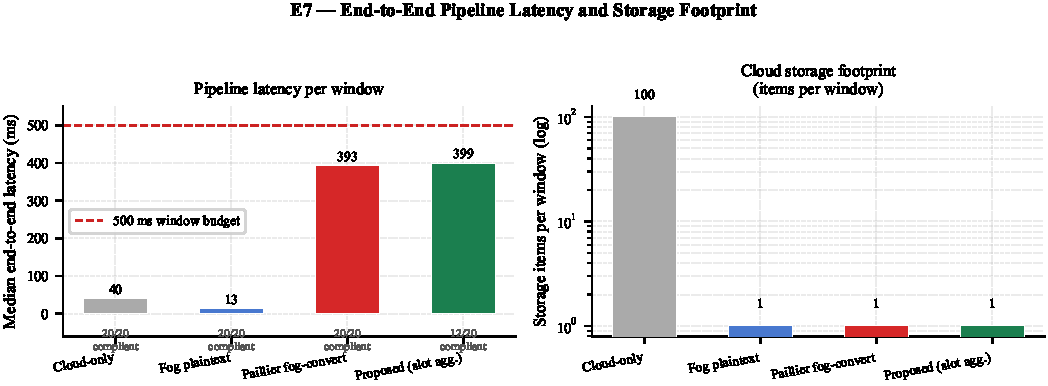
\includegraphics[width=1.0\linewidth]{figures/exp7_pipeline.pdf}
    \caption{E7: Analytical end-to-end pipeline latency (left) and per-window storage items (right) for four methods across 20 windows ($n{=}100$). The dashed line marks the 500~ms window budget. The proposed method exceeds this budget in 8 windows where TEE key delegation is active. \textbf{Note}: This is an analytical model using hardware-target constants; E2 reports a separate calibrated 2048-bit host-reference benchmark.}
    \label{fig:e7-pipeline}
    \end{figure}

    \subsection{E8: Key Exposure Blast Radius}
    \label{sec:eval-e8}

    \textbf{Objective.} Quantify the number of sensors whose decryption key is exposed under four threat scenarios, comparing a global shared AES key architecture with the proposed fog-scoped key design.

    \textbf{Setup.} The system consists of 100 sensors distributed evenly across five fog nodes (20 per node). Four compromise scenarios are evaluated using analytical exposure accounting: (i)~\emph{one fog node compromised} ($F_1$ enclave physically broken); (ii)~\emph{backup node compromised during active delegation} ($F_4$ enclave broken while holding a provisioned $k_{fogA}$ key); (iii)~\emph{KMM compromised}; and (iv)~\emph{host OS reads enclave memory} (under the standard SGX honest-but-curious threat model). These results represent analytical exposure counts and are not the product of a cryptographic attack simulation or SGX penetration test.

    \textbf{Results.} Fig.~\ref{fig:e8-blast} shows the results. In scenario~(i), a global key scheme exposes all 100 sensors while fog-scoped keys expose only the 20 sensors assigned to the compromised node, an 80\% reduction. In scenario~(ii), the backup node holds only $k_{fogA}$ provisioned for the current delegation epoch, exposing 40 sensors (20 from $F_1$ and 20 from $F_4$'s own group) versus all 100 under a global key, a 60\% reduction. In scenario~(iii), KMM compromise exposes all 100 sensors under both schemes, since the KMM is the trust anchor for both; no isolation benefit exists in this scenario. In scenario~(iv), the SGX assumption prevents host OS access to enclave memory in both schemes, so no sensors are exposed under either design.

    \textbf{Key takeaway.} Fog-scoped key isolation reduces sensor exposure by 60--80\% in single-node compromise scenarios relative to a global key design. The benefit does not extend to KMM compromise, which the threat model identifies as a critical single point of failure common to both schemes.

    \begin{figure}[htbp]
    \centering
    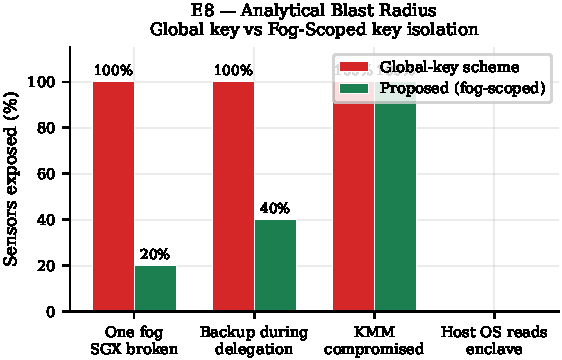
\includegraphics[width=1.0\linewidth]{figures/exp8_blast_radius.pdf}
    \caption{E8: Analytical key exposure comparison between a global AES key design and the proposed fog-scoped key design across four threat scenarios (100 sensors total, 20 per node). KMM compromise exposes all sensors under both schemes.}
    \label{fig:e8-blast}
    \end{figure}

    \section{Future Work}

    A limitation of the present work is that the CapacityScore (S6) weights $(w_1, w_2, w_3, w_4)$ and the compatibility term coefficients are fixed heuristics selected by task classification rather than learned from observed workload distributions. The strategy comparison in E5 demonstrates the advantage of the compatibility-aware term over simpler scoring strategies, but the specific weight values motivate data-driven adaptation. An important direction for future work is to replace the static weight table with an online learning mechanism---such as a contextual bandit or lightweight reinforcement learning policy---that adjusts weights based on observed deadline miss rates and node utilization histories across aggregation windows. Additionally, the workload update model in E5 uses a formula-based service time derived from static node profiles rather than a principled queuing model; extending the simulation to a discrete-event framework with explicit queue dynamics (e.g., M/M/$c$ per node) would produce more accurate estimates of redelegation rates and deadline miss probabilities at larger scales. The present evaluation covers five fog nodes, 20 windows, and 46--58 tasks per window depending on the stress phase; characterizing system behavior under hundreds of nodes and high-variance arrival rates represents a necessary step toward deployment-scale validation. Furthermore, the current Paillier-based aggregation layer supports only additive operations---sum, mean, and weighted sum. Future work will extend the scheme to CKKS-based slot batching to support multiplicative aggregation functions such as variance, product aggregation, and nonlinear statistics, and to provide approximate arithmetic over packed sensor vectors with formally bounded noise growth.

    The experimental evaluation rests on several simplifying assumptions that limit direct correspondence to real deployments. The SGX trusted execution environment is entirely simulated: \texttt{sgx\_enclave\_process} is implemented as an ordinary Python function performing AES decryption followed by Paillier encryption, with no actual enclave boundary, no sealing key derivation, and no remote attestation exchange. The KMM provisioning latency $T_{KMM}=50\,\text{ms}$ is a fixed design parameter rather than a measured quantity. Future work should implement the enclave layer using a real SGX SDK (e.g., Intel SGX SDK or Gramine) and validate provisioning latency on Skylake or Ice Lake class hardware. Similarly, the end-to-end pipeline latency in E7 is derived entirely from hardcoded hardware-target constants; these estimates should be replaced by measurements on physical fog hardware equipped with AES-NI and an SGX-capable processor.

    The fault tolerance evaluation in E6 is based on an analytical reading-loss model that counts sensor readings falling within a fixed failure-to-recovery time window under three predetermined failure timings. This model does not capture cascading failures, partial node degradation, network partition effects, or the interaction between simultaneous sensor ACK timeouts and the gossip convergence process. Future work should validate the proposed ACK+KMM recovery mechanism under realistic fault injection using network emulation tools such as tc-netem or a containerized testbed, and should extend the failure model to cover correlated multi-node failures and transient network outages. The gossip protocol parameters---fan-out $k{=}3$, miss threshold $r{=}3$, and gossip interval $T_g{=}500\,\text{ms}$---are fixed throughout the evaluation; the probabilistic detection model derived from the Poisson failure process provides a design criterion ($T_g \leq \ln(20)/(\mu r)$ for $\beta=0.95$), but adaptive parameter selection under varying failure rates $\mu$ has not been investigated. The KMM is currently modeled as a single trusted authority; future work may investigate threshold or multi-party key management constructions that distribute the trust anchor across a quorum of KMM instances, reducing the exposure when the KMM is compromised. Finally, the present scheme provides computational confidentiality under the IND-CPA assumption for Paillier and AES-GCM but does not address what an honest-but-curious cloud observer can infer from the sequence of decrypted aggregates over time. Investigating differential privacy mechanisms for the aggregate output, or bounding the statistical leakage of the published aggregate stream, remains an open problem for future work.

    \section{Conclusion}

    This paper presented a fault-tolerant and load-balanced IIoT edge--fog architecture that jointly addresses three critical challenges: resource imbalance across heterogeneous fog nodes, fog-layer failures, and plaintext exposure during aggregation. The proposed framework integrates fog-scoped AES key isolation enforced by Intel SGX trusted execution environments, Paillier homomorphic slot aggregation with a zero-fill protocol for mid-window delegation, a three-layer fault-handling hierarchy combining per-reading TEE delegation, sensor ACK-timeout redirect, and gossip-based failure detection, and a task-aware CapacityScore selector that adapts routing decisions to the computational profile of each task type.

    Experimental evaluation across eight experiments demonstrated: constant per-window cloud storage independent of sensor count (E1); aggregate correctness under mid-window delegation in all 100 trials tested (E3); the highest deadline satisfaction rate of 78.77\% and the lowest bandwidth-utilization variance among six compared strategies (E5); worst-case data loss reduced from 75\% under gossip-only detection to 7.5\% with the ACK+KMM mechanism at only $1.055\times$ message overhead (E6); and 60--80\% reduction in key-exposure blast radius relative to a global-key design under single-node compromise (E8).

    Future work will focus on validating the SGX enclave implementation on physical hardware, replacing the static CapacityScore weight table with an adaptive online learning policy, and extending the Paillier aggregation layer to CKKS-based slot batching for multiplicative and nonlinear aggregation functions.

    \bibliographystyle{IEEEtran}
    \bibliography{references}

    \end{document}
